\chapter{Lie群}
\label{chap:lie-groups}

把一组三维点整体转一个角度，点之间的距离不变，表示朝向的向量却跟着转动。把这组点重新编号，空间中的点一个也没有移动，记录点的矩阵却换了行序。要说清某个计算结果“不受旋转影响”还是“随旋转同步变化”，先要知道允许哪些变换、它们怎样接连施加和撤销、每个变换作用在什么对象上。

另一方面，三维朝向由九个矩阵元素记录，却只有三个自由度。两张旋转矩阵的平均通常不再是旋转矩阵，直接在矩阵元素上做加减会破坏约束。第~\ref{chap:manifold-relations}章告诉我们，旋转矩阵组成一个弯曲的子流形；本章要进一步利用“旋转可以复合”这一事实，在这个弯曲的集合上做计算。

这两类问题都要求把变换的复合规则本身当作研究对象。第~\ref{sec:lie-groups}节用置换、平移和旋转的复合建立群、子群与同态。第~\ref{sec:lie-actions}节规定同一个群怎样作用在不同对象上，用轨道和稳定子描述“能到哪里”和“哪些变换不起作用”，再定义不变映射与等变映射。

旋转可以连续地变化，所以第~\ref{sec:lie-matrix-groups}节把矩阵群看成流形：单位元处的切空间即Lie代数，记录无穷小变化，矩阵指数把这些方向变回群中的变换。第~\ref{sec:lie-rotations}节围绕同一个三维旋转比较旋转矩阵、轴角与单位四元数，第~\ref{sec:lie-rigid-poses}节加入平移，建立刚体位姿的计算规则。

最后，第~\ref{sec:lie-quotients}节处理“多种记录代表同一对象”的问题：用群作用把等价的记录合并，说明何时得到光滑的商流形，并建立射影空间与Grassmann空间。

本章依赖第~\ref{chap:manifold-basics}章的流形与切空间、第~\ref{chap:manifold-maps}章的光滑映射与微分、第~\ref{chap:manifold-relations}章的正则水平集，以及第~\ref{chap:topological-spaces}章的商拓扑。由对应点实际估计旋转、平移和射影变换是第~\ref{chap:spatial-map-estimation}章的任务；正交矩阵与子空间约束下的优化算法见\BookChapterRef{chap:manifold-optimization}{卷五第12章“流形约束下的优化”}。

\section{群}
\label{sec:lie-groups}

重新排列三个物品的位置、把平面整体平移一段距离、把平面绕原点转一个角度，这三类操作作用的对象各不相同，却遵循同样的规则：两个操作可以接连施加，得到的仍是同类操作；“什么都不做”也算一个操作；每个操作都可以撤销。本节先把这些规则从具体对象中抽出来，建立群、子群与同态。这里只固定变换之间怎样复合，同一个群怎样作用在不同对象上留给第~\ref{sec:lie-actions}节，这样就不会把一个群只理解成某一套坐标矩阵。

\subsection{群与子群}
\label{sec:lie-group-subgroup}

本小节先从置换的复合读出群公理，再看几类基本例子和反例，最后研究限制允许变换得到的子群。

\paragraph{从变换的复合到群公理}
先看集合$\{1,2,3\}$上的置换，即从这个集合到自身的双射。置换$\sigma$交换$1$与$2$、保持$3$不动，置换$\tau$交换$2$与$3$、保持$1$不动。复合$\sigma\circ\tau$表示先做$\tau$、再做$\sigma$：
\[
(\sigma\circ\tau)(1)=\sigma(1)=2,\qquad
(\sigma\circ\tau)(2)=\sigma(3)=3,\qquad
(\sigma\circ\tau)(3)=\sigma(2)=1.
\]
反过来先做$\sigma$再做$\tau$，得到$1\mapsto3$、$2\mapsto1$、$3\mapsto2$。两个结果不同，所以复合的次序必须写清。

这个例子已经包含群的全部要素。两个置换的复合仍是置换；恒等置换$\operatorname{id}$不改变任何元素；每个置换都有逆置换，把它的效果撤销；映射的复合满足结合律$(\alpha\circ\beta)\circ\gamma=\alpha\circ(\beta\circ\gamma)$，因为两边在每个元素上都等于$\alpha(\beta(\gamma(i)))$。平面上的平移$\bm x\mapsto\bm x+\bm a$和绕原点的旋转同样满足这四条，只是平移的复合对应向量相加，旋转的复合对应转角相加。

\begin{definition}[群]
\label{def:lie-group}
设$G$是集合，$G\times G\to G$，$(g,h)\mapsto gh$是$G$上的二元运算。若
\begin{enumerate}
 \item 对所有$g,h,k\in G$，$(gh)k=g(hk)$；
 \item 存在$e\in G$，使对所有$g\in G$，$eg=ge=g$；
 \item 对每个$g\in G$，存在$g^{-1}\in G$，使$gg^{-1}=g^{-1}g=e$，
\end{enumerate}
就称$G$连同这个运算构成\term{群}（group），$e$称为单位元，$g^{-1}$称为$g$的逆元。若还对所有$g,h$有$gh=hg$，就称$G$为\term{交换群}（commutative group）。
\end{definition}

运算“封闭”已经写在$G\times G\to G$之中：乘积必须仍在$G$里。乘法记号$gh$只是约定，它可以是映射的复合、数的加法或矩阵乘法。对由变换组成的群，本章总按复合约定$gh=g\circ h$，即先做$h$、再做$g$。

\paragraph{几个基本例子}
$\{1,\ldots,n\}$上全部置换在复合下构成群，称为\term{对称群}（symmetric group），记为$S_n$，它有$n!$个元素。上面的计算说明$S_3$不是交换群。$\mathbb R^d$在向量加法下构成交换群，单位元是$\bm0$，逆元是$-\bm a$；它记录平面或空间中的全部平移。

平面旋转由矩阵
\begin{equation}
 \bm R(\theta)=\begin{bmatrix}\cos\theta&-\sin\theta\\\sin\theta&\cos\theta\end{bmatrix}
 \label{eq:lie-planar-rotation}
\end{equation}
表示。由和角公式，$\bm R(\theta_1)\bm R(\theta_2)=\bm R(\theta_1+\theta_2)$，所以平面旋转的复合与次序无关，单位元是$\bm R(0)=\bm I$，逆元是$\bm R(-\theta)=\bm R(\theta)^\top$。

更一般的矩阵例子如下。全体$n$阶可逆实矩阵在矩阵乘法下构成\term{一般线性群}（general linear group），记为$\mathrm{GL}(n,\mathbb R)$。满足$\bm Q^\top\bm Q=\bm I$的正交矩阵构成\term{正交群}（orthogonal group）$\mathrm O(n)$：若$\bm Q_1,\bm Q_2$正交，则$(\bm Q_1\bm Q_2)^\top\bm Q_1\bm Q_2=\bm Q_2^\top\bm Q_2=\bm I$，且$\bm Q^{-1}=\bm Q^\top$仍正交。正交矩阵的行列式为$\pm1$，其中行列式为$1$的构成\term{特殊正交群}（special orthogonal group）$\mathrm{SO}(n)$。当$n=2$时，$\mathrm{SO}(2)$恰由式~\eqref{eq:lie-planar-rotation}中的矩阵组成：第一列$(a,b)^\top$是单位向量，第二列与它正交且使行列式为$1$，只能是$(-b,a)^\top$，再记$a=\cos\theta$、$b=\sin\theta$即可。

\paragraph{不构成群的情形}
公理中的每一条都会实际排除一些对象。全体$n$阶实矩阵在乘法下不是群，因为奇异矩阵没有逆；把一个向量投影到某条直线上的操作不可撤销，同样不能放进群里。整数在减法下不是群，因为$(1-2)-3\neq1-(2-3)$，结合律失败。若一组图像增强操作接连施加后不再属于这一组，运算不封闭，也不能直接称为群。

单位元和逆元一旦存在就是唯一的，因此记号$e$与$g^{-1}$没有歧义。

\begin{lemma}[单位元与逆元的唯一性]
\label{lem:lie-identity-inverse-unique}
群$G$中单位元唯一；每个$g\in G$的逆元唯一。并且对任意$g,h\in G$，$(gh)^{-1}=h^{-1}g^{-1}$。
\end{lemma}

\begin{proof}
若$e,e'$都是单位元，则$e=ee'=e'$。若$h,h'$都是$g$的逆元，则$h=he=h(gh')=(hg)h'=eh'=h'$。最后，由结合律，$(gh)(h^{-1}g^{-1})=g(hh^{-1})g^{-1}=gg^{-1}=e$，另一侧同理，所以$h^{-1}g^{-1}$是$gh$的逆元。
\end{proof}

最后一式的次序与直觉一致：先穿袜子再穿鞋，撤销时要先脱鞋再脱袜子。对矩阵而言，这就是$(\bm A\bm B)^{-1}=\bm B^{-1}\bm A^{-1}$。

\paragraph{子群}
许多问题只允许一部分变换。例如只允许转$90^\circ$的整数倍，或只允许沿水平方向平移。这些变换自身仍然能复合和撤销，于是在原来的群中又形成一个群。

\begin{definition}[子群]
\label{def:lie-subgroup}
设$G$是群，$H\subseteq G$。若$e\in H$，并且对任意$g,h\in H$都有$gh\in H$与$g^{-1}\in H$，就称$H$是$G$的\term{子群}（subgroup）。
\end{definition}

子群继承了原来的运算，结合律自动成立，所以它本身是群。验证子群时，常把三个条件合成一条。

\begin{lemma}[子群判别]
\label{lem:lie-subgroup-criterion}
群$G$的非空子集$H$是子群，当且仅当对任意$g,h\in H$都有$gh^{-1}\in H$。
\end{lemma}

\begin{proof}
必要性由定义直接得到。反过来，取$g\in H$，令$h=g$得$e=gg^{-1}\in H$；再取第一个元素为$e$，得$h^{-1}=eh^{-1}\in H$；最后对$g,h\in H$，由$h^{-1}\in H$得$gh=g(h^{-1})^{-1}\in H$。
\end{proof}

转$90^\circ$整数倍的旋转$\{\bm R(k\pi/2):k=0,1,2,3\}$是$\mathrm{SO}(2)$的子群，它只有四个元素。水平平移$\{(a,0)^\top:a\in\mathbb R\}$是$\mathbb R^2$的子群。矩阵群之间有包含链$\mathrm{SO}(n)\subseteq\mathrm O(n)\subseteq\mathrm{GL}(n,\mathbb R)$，每一个都是后一个的子群。

\paragraph{子集与子群的区别}
子群是“允许的变换”组成的子集，并且对群运算封闭；它不同于被变换对象的一个子集，也不同于群的任意子集。在平移群$\mathbb R^2$中，单位圆$\{\bm x:\lVert\bm x\rVert_2=1\}$是一个子集，却不是子群：$(1,0)^\top+(1,0)^\top=(2,0)^\top$不在圆上，零向量也不在圆上。

同样，$\mathrm O(n)$中行列式为$-1$的矩阵（反射类变换）组成的子集不是子群：它不含$\bm I$，两个反射的乘积行列式为$1$，又回到了旋转。可见“满足某个条件的变换”能否形成子群，要逐条核对单位元、乘积和逆元，不能只看条件写起来是否自然。

\subsection{群同态}
\label{sec:lie-homomorphism}

同一套变换规则可以用不同方式记录。平面旋转可以用转角$\theta$记录，也可以用矩阵$\bm R(\theta)$记录；三个物品的置换可以写成映射表，也可以写成置换矩阵。要说明两种记录描述的是同一个复合结构，需要一个保持复合的映射。

\begin{definition}[群同态与同构]
\label{def:lie-homomorphism}
设$G,H$是群。映射$\varphi:G\to H$若对所有$g_1,g_2\in G$满足
\begin{equation}
 \varphi(g_1g_2)=\varphi(g_1)\varphi(g_2),
 \label{eq:lie-homomorphism}
\end{equation}
就称为\term{群同态}（group homomorphism）。双射的群同态称为\term{群同构}（group isomorphism）。同态的\term{核}（kernel）是$\ker\varphi=\{g\in G:\varphi(g)=e_H\}$，像是$\varphi(G)=\{\varphi(g):g\in G\}$。
\end{definition}

式~\eqref{eq:lie-homomorphism}左边先在$G$中复合再映过去，右边先映过去再在$H$中复合，二者相等。由$\varphi(e_G)=\varphi(e_Ge_G)=\varphi(e_G)\varphi(e_G)$，两边左乘$\varphi(e_G)^{-1}$得$\varphi(e_G)=e_H$；再由$\varphi(g)\varphi(g^{-1})=\varphi(e_G)=e_H$得$\varphi(g^{-1})=\varphi(g)^{-1}$。所以同态自动保持单位元与逆元。

\paragraph{同态的例子}
由式~\eqref{eq:lie-planar-rotation}定义的$\theta\mapsto\bm R(\theta)$是从加法群$\mathbb R$到$\mathrm{SO}(2)$的同态，因为$\bm R(\theta_1+\theta_2)=\bm R(\theta_1)\bm R(\theta_2)$。它是满射，核为$\{2\pi k:k\in\mathbb Z\}$：转角相差$2\pi$的整数倍，得到同一个旋转。

行列式给出同态$\det:\mathrm{GL}(n,\mathbb R)\to\mathbb R\setminus\{0\}$，后者取数的乘法，因为$\det(\bm A\bm B)=\det\bm A\det\bm B$。它的核是行列式为$1$的矩阵全体，记为$\mathrm{SL}(n,\mathbb R)$。

对$\pi\in S_n$，令置换矩阵$\bm P_\pi$的第$j$列为$\bm e_{\pi(j)}$，即$\bm P_\pi\bm e_j=\bm e_{\pi(j)}$。于是
\[
\bm P_{\pi_1}\bm P_{\pi_2}\bm e_j=\bm P_{\pi_1}\bm e_{\pi_2(j)}=\bm e_{\pi_1(\pi_2(j))}=\bm P_{\pi_1\pi_2}\bm e_j,
\]
所以$\pi\mapsto\bm P_\pi$是从$S_n$到$\mathrm{GL}(n,\mathbb R)$的同态，像落在$\mathrm O(n)$中。不同置换给出不同矩阵，这个同态是单射。

把群的复合规则落实为可逆线性映射，是比较各种表示时最常用的同态，下面单独命名。

\begin{definition}[线性表示]
\label{def:lie-linear-representation}
设$G$是群，$V$是有限维实向量空间，$\mathrm{GL}(V)$是$V$上全部可逆线性映射在复合下构成的群。群同态$\rho:G\to\mathrm{GL}(V)$称为$G$在$V$上的\term{线性表示}（linear representation）。
\end{definition}

同一个群可以有许多线性表示。$\mathrm{SO}(2)$可以按$\rho(\bm R)=\bm R$作用在$\mathbb R^2$上，也可以按$\rho(\bm R)=1$作用在$\mathbb R$上，后者把每个旋转都表示为“不做任何事”。第~\ref{sec:lie-invariant-equivariant}节会用这两种表示区分不变与等变。

\paragraph{核与像保留什么}
核记录同态把哪些元素“看成单位元”，因而丢失了哪些区分；像记录目标群中有哪些元素被实际表示出来。下面的结论说明，核只含单位元时同态不丢失任何区分。

\begin{theorem}[核与单射]
\label{thm:lie-kernel-injective}
设$\varphi:G\to H$是群同态。则$\ker\varphi$是$G$的子群，$\varphi(G)$是$H$的子群，并且$\varphi(g_1)=\varphi(g_2)$当且仅当$g_1^{-1}g_2\in\ker\varphi$。特别地，$\varphi$是单射当且仅当$\ker\varphi=\{e_G\}$。
\end{theorem}

\begin{proof}
若$g,h\in\ker\varphi$，则$\varphi(gh^{-1})=\varphi(g)\varphi(h)^{-1}=e_H$，由引理~\ref{lem:lie-subgroup-criterion}知核是子群；对像中的$\varphi(g),\varphi(h)$，有$\varphi(g)\varphi(h)^{-1}=\varphi(gh^{-1})$仍在像中，所以像也是子群。其次，$\varphi(g_1)=\varphi(g_2)$等价于$e_H=\varphi(g_1)^{-1}\varphi(g_2)=\varphi(g_1^{-1}g_2)$，即$g_1^{-1}g_2\in\ker\varphi$。最后，若核只含$e_G$，则$\varphi(g_1)=\varphi(g_2)$推出$g_1^{-1}g_2=e_G$，即$g_1=g_2$；反之，单射把$e_G$之外的元素都映到$e_H$之外。
\end{proof}

回到转角的例子：$\varphi(\theta)=\bm R(\theta)$的核是$2\pi\mathbb Z$，所以$\bm R(\theta_1)=\bm R(\theta_2)$当且仅当$\theta_2-\theta_1\in2\pi\mathbb Z$。转角能完整记录旋转的复合，却在每个旋转上多出可数个等价的记录；第~\ref{sec:lie-rotations}节的轴角与四元数会遇到同类的冗余。

\paragraph{结构对应与集合对应}
两个群元素个数相同，只说明它们之间有集合层面的双射，不说明复合规则相同。$S_3$有$6$个元素，$\{0,1,\ldots,5\}$在模$6$加法下也构成$6$个元素的群，二者之间当然有双射。但模$6$加法群是交换群，$S_3$不是；若$\varphi$是同构，则$\varphi(\sigma)\varphi(\tau)=\varphi(\tau)\varphi(\sigma)$，由单射性得$\sigma\tau=\tau\sigma$，与本节开头的计算矛盾。所以这两个群不同构。

另一方面，平面旋转$\bm R(\theta)$与单位圆上的点$(\cos\theta,\sin\theta)^\top$一一对应。只有给单位圆指定运算，例如把点看成单位复数$e^{\mathrm i\theta}$并取复数乘法，这个对应才成为群同构。判断两种记录是否表达同一个变换结构，要检查的是复合规则是否被保持，而不只是元素能否配对。

\section{群作用}
\label{sec:lie-actions}

上一节的群只规定了变换之间怎样复合。同一个旋转可以转动一个点、一整组点，也可以转动一幅定义在平面上的图像；被变换的对象不同，计算公式也不同。本节先规定群元素怎样作用在给定集合上，并核对作用与复合相容；再用轨道与稳定子描述对象之间通过变换建立的关系；最后在输入与输出的作用都给定后，说明映射的结果应怎样随输入变换。

\begin{definition}[群作用]
\label{def:lie-group-action}
设$G$是群，$X$是集合。映射$G\times X\to X$，$(g,x)\mapsto g\cdot x$若满足
\begin{equation}
 e\cdot x=x,\qquad (g_1g_2)\cdot x=g_1\cdot(g_2\cdot x)\qquad(g_1,g_2\in G,\ x\in X),
 \label{eq:lie-group-action}
\end{equation}
就称为$G$在$X$上的\term{群作用}（group action）。
\end{definition}

第一条说单位元什么也不做，第二条说先用$g_2$作用、再用$g_1$作用，与用乘积$g_1g_2$作用一次相同。对固定的$g$，映射$x\mapsto g\cdot x$有逆映射$x\mapsto g^{-1}\cdot x$，因为$g^{-1}\cdot(g\cdot x)=(g^{-1}g)\cdot x=x$。所以群作用相当于一个同态，把每个$g$对应为$X$上的一个双射。

\paragraph{同一个群在不同对象上的作用}
$\mathrm{SO}(2)$在$\mathbb R^2$上按矩阵乘法$\bm R\cdot\bm x=\bm R\bm x$作用，两条规则就是$\bm I\bm x=\bm x$与矩阵乘法的结合律。$\mathbb R^2$也按$\bm a\cdot\bm x=\bm x+\bm a$作用在自身上。

点云由$n$个点组成，记为$\bm X\in\mathbb R^{n\times D}$，第$i$行$\bm X_{i,:}$是第$i$个点的坐标。$S_n$按$\pi\cdot\bm X=\bm P_\pi\bm X$作用，其中$\bm P_\pi$沿用上一节的置换矩阵；由$\bm P_\pi\bm e_j=\bm e_{\pi(j)}$可以算出$(\bm P_\pi\bm X)_{i,:}=\bm X_{\pi^{-1}(i),:}$，即原来的第$j$行被搬到第$\pi(j)$行。$\mathrm{SO}(D)$则按$\bm R\cdot\bm X=\bm X\bm R^\top$作用，把每一行$\bm x^\top$变成$(\bm R\bm x)^\top$。两种作用都写成矩阵乘法，前者改变点的编号，后者移动点的位置，被改变的对象和索引完全不同。

旋转还可以作用在平面图像上。把图像记为函数$f:\mathbb R^2\to\mathbb R$，令
\[
(\bm R\cdot f)(\bm x)=f(\bm R^{-1}\bm x).
\]
这里必须用$\bm R^{-1}$：新图像在$\bm x$处的值，来自旧图像中转到$\bm x$之前的位置。验证第二条规则：$(\bm R_1\cdot(\bm R_2\cdot f))(\bm x)=(\bm R_2\cdot f)(\bm R_1^{-1}\bm x)=f(\bm R_2^{-1}\bm R_1^{-1}\bm x)=f((\bm R_1\bm R_2)^{-1}\bm x)$，恰为$((\bm R_1\bm R_2)\cdot f)(\bm x)$。若改写成$f(\bm R\bm x)$，复合次序就会颠倒，在非交换群上不再满足式~\eqref{eq:lie-group-action}。

\subsection{轨道与稳定子}
\label{sec:lie-orbits-stabilizers}

给定作用后，可以问两个方向相反的问题：从一个对象出发，经过群中的变换能到达哪些对象；哪些变换根本不改变这个对象。前者给出轨道，后者给出稳定子。

\begin{definition}[轨道与稳定子]
\label{def:lie-orbit-stabilizer}
设群$G$作用于$X$，$x\in X$。称
\[
G\cdot x=\{g\cdot x:g\in G\},\qquad G_x=\{g\in G:g\cdot x=x\}
\]
分别为$x$的\term{轨道}（orbit）与\term{稳定子}（stabilizer）。若$X$只有一条轨道，就称作用是\term{传递作用}（transitive action）。
\end{definition}

轨道是$X$的子集，稳定子是$G$的子集，二者不在同一个空间里。规定$x\sim y$当且仅当存在$g\in G$使$y=g\cdot x$。单位元给出$x\sim x$；若$y=g\cdot x$，则$x=g^{-1}\cdot y$，给出对称性；若$y=g\cdot x$、$z=h\cdot y$，则$z=(hg)\cdot x$，给出传递性。所以$\sim$是等价关系，其等价类恰是轨道。由等价关系与划分的对应（可参考\BookChapterRef{chap:sets-relations-maps}{卷一第1章“集合、关系与映射”}），不同的轨道互不相交，且所有轨道的并是$X$。轨道组成的商集记为$X/G$。

稳定子则总是子群。若$g,h\in G_x$，则$h^{-1}\cdot x=h^{-1}\cdot(h\cdot x)=x$，于是$(gh^{-1})\cdot x=g\cdot(h^{-1}\cdot x)=x$，由引理~\ref{lem:lie-subgroup-criterion}得$G_x$是子群。

\paragraph{旋转作用的轨道}
$\mathrm{SO}(2)$作用于$\mathbb R^2$时，$\bm x\neq\bm0$的轨道是半径为$\lVert\bm x\rVert_2$的圆：旋转保持长度，并且同一圆上任意两点之间都有一个旋转把一点送到另一点。原点的轨道只有原点自身。非零点的稳定子只含$\bm I$，原点的稳定子是整个$\mathrm{SO}(2)$。轨道可以用半径$r\geq0$编号，所以$\mathbb R^2/\mathrm{SO}(2)$可以识别为$[0,\infty)$，原点的轨道对应端点$0$。

$\mathrm{SO}(3)$作用于$\mathbb R^3$时，非零点的轨道是球面。以$\bm e_3=(0,0,1)^\top$为例，它的轨道是单位球面$S^2$，稳定子是绕第三坐标轴的全部旋转
\[
\left\{\begin{bmatrix}\bm R(\theta)&\bm0\\\bm0^\top&1\end{bmatrix}:\theta\in\mathbb R\right\},
\]
这是一个与$\mathrm{SO}(2)$同构的子群。这里有三个不同的空间：群$\mathrm{SO}(3)$由旋转组成，单个对象$\bm e_3$是一个点，轨道$S^2$是一个曲面。许多不同的旋转把$\bm e_3$送到同一个点，所以不能把$\mathrm{SO}(3)$与球面$S^2$等同；第~\ref{sec:lie-quotients}节会说明$S^2$正是$\mathrm{SO}(3)$按这个稳定子取商的结果。

\paragraph{轨道与陪集}
两个变换把$x$送到同一个点，当且仅当它们只差一个稳定子中的元素：$g\cdot x=h\cdot x$等价于$(h^{-1}g)\cdot x=x$，即$h^{-1}g\in G_x$。为了记录“只差$G_x$中元素”的变换，引入下面的集合。

\begin{definition}[陪集]
\label{def:lie-coset}
设$H$是群$G$的子群，$g\in G$。称$gH=\{gh:h\in H\}$为$H$的一个左\term{陪集}（coset）。全体左陪集组成的集合记为$G/H$。
\end{definition}

$h^{-1}g\in G_x$恰等价于$g\in hG_x$，于是$gG_x=hG_x$当且仅当$g\cdot x=h\cdot x$。这说明映射$gG_x\mapsto g\cdot x$不依赖代表元，并且是从$G/G_x$到轨道$G\cdot x$的双射。

\begin{theorem}[轨道—稳定子关系]
\label{thm:lie-orbit-stabilizer}
设群$G$作用于$X$，$x\in X$。则$gG_x\mapsto g\cdot x$是$G/G_x$到$G\cdot x$的双射。若$G$是有限群，则$\lvert G\cdot x\rvert\,\lvert G_x\rvert=\lvert G\rvert$。
\end{theorem}

\begin{proof}
双射已在上一段证明。有限情形下，左乘$g$是$G$到自身的双射，把$G_x$一一地映成$gG_x$，所以每个陪集都有$\lvert G_x\rvert$个元素。不同陪集互不相交：若$k\in gG_x\cap hG_x$，则$k\cdot x=g\cdot x=h\cdot x$，从而$gG_x=hG_x$。每个$g$都在自己的陪集$gG_x$中，所以$G$被分成$\lvert G/G_x\rvert=\lvert G\cdot x\rvert$个大小为$\lvert G_x\rvert$的块。
\end{proof}

用$S_3$作用于$\{1,2,3\}$核对：$1$的轨道是$\{1,2,3\}$，稳定子是$\{\operatorname{id},\tau\}$，其中$\tau$交换$2$与$3$，确有$3\times2=6$。对点云，若$\bm X$的$n$行互不相同，则只有恒等置换保持$\bm X$，轨道有$n!$个元素，对应同一组点的$n!$种编号方式；若恰有两行相同，交换这两行也保持$\bm X$，稳定子有$2$个元素，轨道只有$n!/2$个不同的矩阵。

\subsection{不变映射与等变映射}
\label{sec:lie-invariant-equivariant}

在点云上计算一个量时，任务往往对变换有明确要求。点的重新编号不应改变“这组点的重心在哪里”；整体旋转之后，重心应跟着转到新的位置，而点之间的距离则不应改变。两种要求都是在比较“变换后再计算”与“计算后再变换”，区别在于输出是否也受到作用。

\begin{definition}[不变映射与等变映射]
\label{def:lie-invariant-equivariant}
设群$G$作用于$X$与$Y$，映射$f:X\to Z$，$F:X\to Y$。若
\begin{equation}
 f(g\cdot x)=f(x)\qquad(g\in G,\ x\in X),
 \label{eq:lie-invariant}
\end{equation}
就称$f$是\term{不变映射}（invariant map）。若
\begin{equation}
 F(g\cdot x)=g\cdot F(x)\qquad(g\in G,\ x\in X),
 \label{eq:lie-equivariant}
\end{equation}
就称$F$是\term{等变映射}（equivariant map），其中左边的点是$X$上的作用，右边的点是$Y$上的作用。
\end{definition}

不变性只需要输入的作用；等变性必须同时给定输入与输出的作用，否则式~\eqref{eq:lie-equivariant}没有意义。若$Y$上的作用是平凡作用$g\cdot y=y$，等变就退化为不变。所以不变是等变的特例，而不是另一种更强或更好的要求。

\paragraph{同一次变换下的核对}
取$\bm x=(1.3,0.5)^\top$，绕原点逆时针转$90^\circ$，$\bm R(\pi/2)\bm x=(-0.5,1.3)^\top$。长度$f(\bm x)=\lVert\bm x\rVert_2$在变换前后都等于$\sqrt{1.94}$，满足式~\eqref{eq:lie-invariant}。恒等映射$F(\bm x)=\bm x$满足$F(\bm R\bm x)=\bm R\bm x=\bm R F(\bm x)$，是等变映射，但$F(\bm R\bm x)=(-0.5,1.3)^\top\neq F(\bm x)$，所以它不是不变映射。等变保留的是“输出随输入同步变化”的规则，而不是输出保持不动。

\paragraph{点云上的例子}
对点云$\bm X\in\mathbb R^{n\times D}$，令$\bm 1\in\mathbb R^n$为全一向量，重心为$\bm m(\bm X)=\frac1n\bm X^\top\bm 1\in\mathbb R^D$。重新编号时，$\bm m(\bm P_\pi\bm X)=\frac1n\bm X^\top\bm P_\pi^\top\bm 1=\bm m(\bm X)$，因为置换矩阵的每一行恰有一个$1$，$\bm P_\pi^\top\bm 1=\bm 1$。旋转时，$\bm m(\bm X\bm R^\top)=\frac1n\bm R\bm X^\top\bm 1=\bm R\,\bm m(\bm X)$。所以重心对置换不变，对旋转等变，输出的旋转作用是$\bm y\mapsto\bm R\bm y$。

两两距离矩阵$\bm D(\bm X)_{i,j}=\lVert\bm X_{i,:}-\bm X_{j,:}\rVert_2$对旋转不变，因为旋转保持差向量的长度。它对置换却不是不变的：重新编号后，$\bm D(\bm P_\pi\bm X)$的$(i,j)$元是原来第$\pi^{-1}(i)$、$\pi^{-1}(j)$两点的距离，即$\bm D(\bm P_\pi\bm X)=\bm P_\pi\bm D(\bm X)\bm P_\pi^\top$。若在矩阵空间上规定作用$\pi\cdot\bm M=\bm P_\pi\bm M\bm P_\pi^\top$，$\bm D$就是等变的。同一个映射是否“对置换不变”，取决于问的是哪一种输出作用。

\paragraph{不变映射与轨道}
不变映射在同一条轨道上取相同的值，所以它只依赖输入所在的轨道。记$q:X\to X/G$为$q(x)=G\cdot x$，令$\widetilde f(G\cdot x)=f(x)$；若$G\cdot x=G\cdot y$，则$y=g\cdot x$，由不变性$f(y)=f(x)$，所以$\widetilde f$不依赖代表元，并且$f=\widetilde f\circ q$。不变映射正是忽略了同一轨道内的差别。

这种忽略可能过多。$f$可以把不同的轨道映到同一个值，例如把每个点云都映到零的常值映射对一切作用都不变，却不区分任何点云。不变性只说明$f$没有利用轨道内的差别，不说明$f$保留了区分不同轨道所需的信息。

\paragraph{复合与汇总}
等变映射之后接不变映射，结果不变：若$F$等变、$f$在$Y$上不变，则$f(F(g\cdot x))=f(g\cdot F(x))=f(F(x))$。两个等变映射的复合仍等变，理由相同。例如对每个点使用同一个映射$\phi:\mathbb R^D\to\mathbb R^r$，令$\Phi(\bm X)_{i,:}=\phi(\bm X_{i,:})$，则$\Phi(\bm P_\pi\bm X)_{i,:}=\phi(\bm X_{\pi^{-1}(i),:})=(\bm P_\pi\Phi(\bm X))_{i,:}$，所以$\Phi$对置换等变；再对行求和，重新编号只改变求和次序，得到不变的$\sum_i\phi(\bm X_{i,:})$。反过来，若中间已经求和，丢掉了每个点的编号，后面就不能再恢复逐点的等变输出。

\section{矩阵Lie群}
\label{sec:lie-matrix-groups}

置换群只有有限个元素，旋转却可以连续地变化：转角从$0$逐渐增大，旋转矩阵也随之连续变化。对这类群，可以问“单位元附近有哪些变化方向”，也可以要求群运算与这些方向的计算相容。本节先说明矩阵群怎样成为流形，并且乘法与求逆都是光滑映射；再用单位元处的切空间记录无穷小变化，即Lie代数；最后用矩阵指数把Lie代数中的方向变回群中的变换。

\begin{definition}[Lie群]
\label{def:lie-lie-group}
若群$G$同时是光滑流形，并且乘法$G\times G\to G$，$(g,h)\mapsto gh$与求逆$G\to G$，$g\mapsto g^{-1}$都是光滑映射，就称$G$为\term{Lie群}（Lie group）。
\end{definition}

定义要求群结构与光滑结构相容，而不只是“元素可以连续变化”。并非每个由连续变换组成的群都是有限维Lie群。例如以有理数倍$2\pi$为转角的旋转$\{\bm R(2\pi q):q\in\mathbb Q\}$是$\mathrm{SO}(2)$的子群，但它只有可数个元素，并且在单位圆上稠密：任意小的弧内都有它的元素。在继承的拓扑下，它的任一点附近既不像一段开区间，也不是孤立点，因而不是流形。圆周上全体同胚组成的群虽然也由连续变换组成，却不能用有限个实数参数局部描述，超出了本章讨论的范围。

本章只讨论矩阵组成的Lie群。称$\mathrm{GL}(n,\mathbb R)$的子群$G$为\term{矩阵Lie群}（matrix Lie group），若$G$在$\mathrm{GL}(n,\mathbb R)$中是闭集。可以证明，$\mathrm{GL}(n,\mathbb R)$的每个闭子群都是嵌入子流形，从而是Lie群（Cartan闭子群定理），这里不给出证明，可参考\scite{math-lee2013smooth}。下面用到的群都直接验证其流形结构，不依赖这个定理。上面的有理转角子群不是闭集，正好被这一定义排除。

\subsection{光滑结构}
\label{sec:lie-smooth-structure}

要把矩阵群当作流形，需要逐一说明它在矩阵空间中是什么样的子集、乘法与求逆为何光滑，以及各点的切空间怎样联系起来。下面依次处理一般线性群、正交群与左平移。

\paragraph{一般线性群}
把$n$阶实矩阵的$n^2$个元素排成一列，$\mathbb R^{n\times n}$就是欧氏空间。行列式是矩阵元素的多项式，因而连续，所以$\mathrm{GL}(n,\mathbb R)=\{\bm A:\det\bm A\neq0\}$是$\mathbb R^{n\times n}$中的开集，从而是$n^2$维流形，一张坐标图就覆盖全体。矩阵乘积的每个元素是两个因子元素的二次多项式，所以乘法光滑。由古典伴随公式$\bm A^{-1}=\operatorname{adj}(\bm A)/\det\bm A$，逆矩阵的元素是矩阵元素的有理函数，分母$\det\bm A$在$\mathrm{GL}(n,\mathbb R)$上不为零，所以求逆光滑。于是$\mathrm{GL}(n,\mathbb R)$是Lie群。

\paragraph{正交群}
正交群由约束$\bm A^\top\bm A=\bm I$给出。用第~\ref{chap:manifold-relations}章的正则水平集判断它是否是子流形时，约束映射的取值空间要选对。令$\mathrm{Sym}(n)$为$n$阶实对称矩阵组成的空间，维数为$n(n+1)/2$，定义
\[
\Phi:\mathrm{GL}(n,\mathbb R)\to\mathrm{Sym}(n),\qquad \Phi(\bm A)=\bm A^\top\bm A.
\]
$\bm A^\top\bm A$本来就对称，若把$\Phi$看成取值于$\mathbb R^{n\times n}$，上三角与下三角的方程会重复，微分不可能满秩。取值于$\mathrm{Sym}(n)$后，$\mathrm O(n)=\Phi^{-1}(\bm I)$。

\begin{theorem}[正交群的流形结构]
\label{thm:lie-orthogonal-group-manifold}
$\mathrm O(n)$是$\mathrm{GL}(n,\mathbb R)$中$n(n-1)/2$维的嵌入子流形，并且对$\bm A\in\mathrm O(n)$，
\begin{equation}
 T_{\bm A}\mathrm O(n)=\{\bm A\bm\Omega:\bm\Omega^\top=-\bm\Omega\}.
 \label{eq:lie-orthogonal-tangent}
\end{equation}
$\mathrm{SO}(n)$是$\mathrm O(n)$中的开子集，具有相同的维数与切空间。
\end{theorem}

\begin{proof}
沿方向$\bm H$求导，$\mathrm d\Phi_{\bm A}(\bm H)=\bm A^\top\bm H+\bm H^\top\bm A$。设$\bm A\in\mathrm O(n)$，任给$\bm S\in\mathrm{Sym}(n)$，取$\bm H=\frac12\bm A\bm S$，则
\[
\mathrm d\Phi_{\bm A}(\bm H)=\tfrac12\bm A^\top\bm A\bm S+\tfrac12\bm S^\top\bm A^\top\bm A=\tfrac12\bm S+\tfrac12\bm S=\bm S,
\]
所以$\mathrm d\Phi_{\bm A}$是满射，$\bm I$是正则值。由正则水平集定理，$\mathrm O(n)$是维数为$n^2-n(n+1)/2=n(n-1)/2$的嵌入子流形，切空间是$\ker\mathrm d\Phi_{\bm A}=\{\bm H:\bm A^\top\bm H\text{反对称}\}$。令$\bm\Omega=\bm A^\top\bm H$，由$\bm A\bm A^\top=\bm I$得$\bm H=\bm A\bm\Omega$，即式~\eqref{eq:lie-orthogonal-tangent}。最后，$\det$在$\mathrm O(n)$上连续且只取$\pm1$，所以$\mathrm{SO}(n)=\mathrm O(n)\cap\{\det>0\}$是$\mathrm O(n)$的开子集。
\end{proof}

$n=3$时维数为$3$，这正是三维朝向的自由度：九个矩阵元素满足六个独立的约束。乘法与求逆在$\mathrm O(n)$上光滑，是因为它们是$\mathrm{GL}(n,\mathbb R)$上光滑映射的限制，并且像仍落在$\mathrm O(n)$中；第~\ref{chap:manifold-relations}章说明，取值于嵌入子流形的光滑映射作为到该子流形的映射也是光滑的。$\mathrm{SL}(n,\mathbb R)=\det^{-1}(1)$可以同样处理：$\mathrm d\det_{\bm I}(\bm H)=\operatorname{tr}\bm H$不恒为零，在一般点上也满秩，所以它是$n^2-1$维的Lie群。

\paragraph{左平移}
式~\eqref{eq:lie-orthogonal-tangent}说明，$\bm A$处的切空间就是把单位元处的切空间整体左乘$\bm A$。这是群结构带来的一般现象。对Lie群$G$中的$g$，称$L_g:G\to G$，$L_g(h)=gh$为\term{左平移}（left translation）。它光滑，并且有光滑逆$L_{g^{-1}}$，所以是微分同胚，它的微分$\mathrm d(L_g)_e:T_eG\to T_gG$是线性同构。对矩阵群，$L_{\bm A}(\bm B)=\bm A\bm B$是线性映射，微分就是$\bm H\mapsto\bm A\bm H$。

因此只要知道单位元处的切空间，就能用群乘法得到任何一点处的切空间。用第~\ref{chap:manifold-basics}章建立的切空间语言，这把一个随点变化的对象化为一个固定的线性空间，下一小节就从这个线性空间入手。

\subsection{Lie代数}
\label{sec:lie-lie-algebra}

设$G$是矩阵Lie群。经过单位元的光滑曲线$\gamma:(-\varepsilon,\varepsilon)\to G$，$\gamma(0)=\bm I$，其速度$\gamma'(0)$是一个$n$阶矩阵，表示在单位元附近变换最先改变的方向。把这些速度全部收集起来，得到单位元处的切空间
\[
\mathfrak g=T_{\bm I}G=\{\gamma'(0):\gamma\text{为}G\text{中光滑曲线},\ \gamma(0)=\bm I\}.
\]
它是$\mathbb R^{n\times n}$的线性子空间。由上一小节，$\mathfrak{gl}(n)=\mathbb R^{n\times n}$是$\mathrm{GL}(n,\mathbb R)$的切空间，$\mathfrak{so}(n)=\{\bm\Omega:\bm\Omega^\top=-\bm\Omega\}$是$\mathrm O(n)$与$\mathrm{SO}(n)$的切空间，$\mathfrak{sl}(n)=\{\bm H:\operatorname{tr}\bm H=0\}$是$\mathrm{SL}(n,\mathbb R)$的切空间。

线性组合在$\mathfrak g$中有明确含义：若$\gamma_1,\gamma_2$是两条经过$\bm I$的曲线，则$\gamma(t)=\gamma_1(a t)\gamma_2(b t)$也在$G$中，由乘积求导得$\gamma'(0)=a\gamma_1'(0)+b\gamma_2'(0)$。所以把两个无穷小变化按比例叠加，对应于把两个小变换接连施加，二者在一阶上相同。

\paragraph{交换子}
接连施加的次序在一阶上看不出来，在二阶上却会显现。旋转一般不交换，Lie代数需要另一个运算记录这种不交换。

\begin{theorem}[交换子封闭]
\label{thm:lie-bracket-closed}
设$G$是矩阵Lie群，$\mathfrak g=T_{\bm I}G$。则对任意$\bm A\in G$与$\bm Y\in\mathfrak g$，有$\bm A\bm Y\bm A^{-1}\in\mathfrak g$；对任意$\bm X,\bm Y\in\mathfrak g$，有
\begin{equation}
 [\bm X,\bm Y]=\bm X\bm Y-\bm Y\bm X\in\mathfrak g.
 \label{eq:lie-commutator}
\end{equation}
\end{theorem}

\begin{proof}
设$\delta$是$G$中经过$\bm I$、速度为$\bm Y$的曲线，则$s\mapsto\bm A\delta(s)\bm A^{-1}$仍是$G$中经过$\bm I$的曲线，速度为$\bm A\bm Y\bm A^{-1}$，第一项得证。再设$\gamma$是速度为$\bm X$的曲线，令$c(t)=\gamma(t)\bm Y\gamma(t)^{-1}$。由第一项，$c(t)$始终落在线性子空间$\mathfrak g$中，所以它的导数也在$\mathfrak g$中。对$\gamma\gamma^{-1}=\bm I$求导得$(\gamma^{-1})'(0)=-\bm X$，于是$c'(0)=\bm X\bm Y-\bm Y\bm X$。
\end{proof}

称$[\bm X,\bm Y]$为\term{交换子}（commutator）。它满足三条规则：对每个变元线性；反对称，$[\bm X,\bm Y]=-[\bm Y,\bm X]$；Jacobi恒等式$[\bm X,[\bm Y,\bm Z]]+[\bm Y,[\bm Z,\bm X]]+[\bm Z,[\bm X,\bm Y]]=\bm0$，后者把三项展开后十二个乘积两两相消即得。一般地，带有满足这三条规则的二元运算的向量空间称为\term{Lie代数}（Lie algebra），矩阵Lie群的切空间$\mathfrak g$连同交换子是它的Lie代数。

\paragraph{与向量场括号的关系}
第~\ref{chap:manifold-basics}章用两个方向导数的交换差定义了向量场的Lie括号，这里的交换子与它一致。在开集$\mathrm{GL}(n,\mathbb R)\subseteq\mathbb R^{n\times n}$上，给定$\bm X$，令$\widetilde{\bm X}(\bm A)=\bm A\bm X$，这是由左平移把$\bm X$搬到每一点得到的向量场。欧氏开集上向量场的括号是$[V,W](\bm A)=\mathrm DW(\bm A)[V(\bm A)]-\mathrm DV(\bm A)[W(\bm A)]$；由$\mathrm D\widetilde{\bm Y}(\bm A)[\bm H]=\bm H\bm Y$，得
\[
[\widetilde{\bm X},\widetilde{\bm Y}](\bm A)=\bm A\bm X\bm Y-\bm A\bm Y\bm X=\bm A[\bm X,\bm Y].
\]
所以交换子正是这些左平移场的括号在单位元处的值。

\paragraph{旋转的Lie代数}
对$\bm\omega=(\omega_1,\omega_2,\omega_3)^\top\in\mathbb R^3$，令
\begin{equation}
 [\bm\omega]_\times=\begin{bmatrix}0&-\omega_3&\omega_2\\\omega_3&0&-\omega_1\\-\omega_2&\omega_1&0\end{bmatrix},
 \qquad [\bm\omega]_\times\bm x=\bm\omega\times\bm x.
 \label{eq:lie-hat-map}
\end{equation}
每个三阶反对称矩阵都唯一地写成这种形式，所以$\bm\omega\mapsto[\bm\omega]_\times$是$\mathbb R^3$到$\mathfrak{so}(3)$的线性同构，三维旋转的无穷小变化由一个三维向量记录。交换子对应叉积：$[[\bm a]_\times,[\bm b]_\times]=[\bm a\times\bm b]_\times$。验证时作用于任意$\bm x$，由二重叉积公式，
\[
\bm a\times(\bm b\times\bm x)-\bm b\times(\bm a\times\bm x)
=\bm b(\bm a^\top\bm x)-\bm a(\bm b^\top\bm x)=(\bm a\times\bm b)\times\bm x.
\]
例如$[[\bm e_1]_\times,[\bm e_2]_\times]=[\bm e_3]_\times$：绕第一轴与绕第二轴的小转动交替进行，二阶上产生绕第三轴的转动。

\paragraph{Lie代数元素与群元素}
Lie代数中的元素是速度，不是变换。$\mathfrak{so}(3)$中的矩阵反对称，而$\mathrm{SO}(3)$中的矩阵正交，二者除了作为矩阵之外没有包含关系：零矩阵在$\mathfrak{so}(3)$中，却不在$\mathrm{SO}(3)$中。Lie代数可以做线性组合，群却不能：$\bm I+\bm I=2\bm I$不是正交矩阵，两个旋转矩阵的平均一般也不是旋转矩阵。要从Lie代数回到群，需要下一小节的矩阵指数。

\subsection{矩阵指数}
\label{sec:lie-matrix-exponential}

给定$\bm X\in\mathfrak g$，我们希望找到一族变换$\gamma(t)\in G$，它以$\bm X$为初速度，并且“转$s$再转$t$等于转$s+t$”，正如$\bm R(\theta)$对转角那样。数的情形下，满足$f(s+t)=f(s)f(t)$、$f'(0)=x$的可微函数是$e^{tx}$。把指数函数的幂级数搬到矩阵上，就得到所需的变换。

\begin{definition}[矩阵指数]
\label{def:lie-matrix-exponential}
对$\bm X\in\mathbb R^{n\times n}$，定义
\begin{equation}
 \exp(\bm X)=\sum_{k=0}^\infty\frac{\bm X^k}{k!}=\bm I+\bm X+\frac{\bm X^2}{2}+\cdots,
 \label{eq:lie-matrix-exponential}
\end{equation}
称为$\bm X$的\term{矩阵指数}（matrix exponential）。
\end{definition}

级数对任意方阵绝对收敛。取一种满足次乘性$\lVert\bm A\bm B\rVert\leq\lVert\bm A\rVert\lVert\bm B\rVert$的矩阵范数，例如谱范数（可参考\BookChapterRef{chap:normed-inner-product-spaces}{卷二第3章“赋范空间与内积空间”}），则$\lVert\bm X^k/k!\rVert\leq\lVert\bm X\rVert^k/k!$，右边是收敛的数项级数$e^{\lVert\bm X\rVert}$。同一估计说明，在$\lVert\bm X\rVert\leq r$上级数一致收敛。对角矩阵的各次幂仍是对角矩阵，所以它的指数就是逐个对角元取指数。

\begin{lemma}[矩阵指数的基本性质]
\label{lem:lie-exponential-properties}
对$\bm X,\bm Y\in\mathbb R^{n\times n}$与可逆矩阵$\bm S$：
\begin{enumerate}
 \item 若$\bm X\bm Y=\bm Y\bm X$，则$\exp(\bm X+\bm Y)=\exp(\bm X)\exp(\bm Y)$；
 \item $\exp(\bm X)$可逆，$\exp(\bm X)^{-1}=\exp(-\bm X)$；
 \item $\exp(\bm X^\top)=\exp(\bm X)^\top$，$\exp(\bm S\bm X\bm S^{-1})=\bm S\exp(\bm X)\bm S^{-1}$；
 \item $t\mapsto\exp(t\bm X)$光滑，且$\frac{\mathrm d}{\mathrm dt}\exp(t\bm X)=\bm X\exp(t\bm X)=\exp(t\bm X)\bm X$；
 \item $\det\exp(\bm X)=e^{\operatorname{tr}\bm X}$。
\end{enumerate}
\end{lemma}

\begin{proof}
（1）$\bm X,\bm Y$交换时二项式定理成立，$(\bm X+\bm Y)^m=\sum_{k+l=m}\frac{m!}{k!\,l!}\bm X^k\bm Y^l$。两个绝对收敛级数的Cauchy乘积可以任意重排，所以
$\exp(\bm X)\exp(\bm Y)=\sum_{m}\sum_{k+l=m}\frac{\bm X^k\bm Y^l}{k!\,l!}=\sum_m\frac{(\bm X+\bm Y)^m}{m!}$。
（2）$\bm X$与$-\bm X$交换，由（1）得$\exp(\bm X)\exp(-\bm X)=\exp(\bm0)=\bm I$。
（3）逐项取转置或共轭，再用$(\bm S\bm X\bm S^{-1})^k=\bm S\bm X^k\bm S^{-1}$与级数的连续性。
（4）$t\bm X$与$h\bm X$交换，由（1）得$\exp((t+h)\bm X)-\exp(t\bm X)=(\exp(h\bm X)-\bm I)\exp(t\bm X)$，而
$\lVert(\exp(h\bm X)-\bm I)/h-\bm X\rVert\leq\sum_{k\geq2}\lvert h\rvert^{k-1}\lVert\bm X\rVert^k/k!\to0$，于是导数为$\bm X\exp(t\bm X)$；$\bm X$与$\exp(t\bm X)$交换，也可写成$\exp(t\bm X)\bm X$。重复这一论证得到各阶导数。
（5）令$f(t)=\det\exp(t\bm X)$。由（1）与行列式的乘法性，$f(t+h)=f(t)\det\exp(h\bm X)$。行列式在$\bm I$处的微分是迹，即$\det(\bm I+\bm H)=1+\operatorname{tr}\bm H+o(\lVert\bm H\rVert)$（可参考\BookChapterRef{chap:matrix-differentiation}{卷二第18章“矩阵函数的微分”}），而$\exp(h\bm X)=\bm I+h\bm X+O(h^2)$，所以$f'(t)=f(t)\operatorname{tr}\bm X$。于是$(e^{-t\operatorname{tr}\bm X}f(t))'=0$，由$f(0)=1$得$f(t)=e^{t\operatorname{tr}\bm X}$，取$t=1$即可。
\end{proof}

交换条件不能去掉。取$\bm X=\begin{bmatrix}0&1\\0&0\end{bmatrix}$、$\bm Y=\begin{bmatrix}0&0\\1&0\end{bmatrix}$，二者的平方都是零矩阵，所以$\exp(\bm X)=\bm I+\bm X$、$\exp(\bm Y)=\bm I+\bm Y$，乘积为$\begin{bmatrix}2&1\\1&1\end{bmatrix}$。而$\bm X+\bm Y$的平方是$\bm I$，按奇偶项汇总得$\exp(\bm X+\bm Y)=\cosh1\,\bm I+\sinh1\,(\bm X+\bm Y)$，对角元是$\cosh1\approx1.543\neq2$。

\paragraph{单参数子群}
由性质（1），$\exp((s+t)\bm X)=\exp(s\bm X)\exp(t\bm X)$，所以$t\mapsto\exp(t\bm X)$是从加法群$\mathbb R$到$\mathrm{GL}(n,\mathbb R)$的光滑同态，初速度为$\bm X$。这样的同态称为\term{单参数子群}（one-parameter subgroup）。下面的结论说明，初速度完全决定了单参数子群。

\begin{theorem}[单参数子群由初速度决定]
\label{thm:lie-one-parameter-subgroup}
设$\gamma:\mathbb R\to\mathrm{GL}(n,\mathbb R)$可微，$\gamma(s+t)=\gamma(s)\gamma(t)$对所有$s,t$成立，且$\gamma'(0)=\bm X$。则$\gamma(t)=\exp(t\bm X)$。
\end{theorem}

\begin{proof}
同态性给出$\gamma(0)=\bm I$与$\gamma(t+h)=\gamma(h)\gamma(t)$，所以$\gamma'(t)=\lim_{h\to0}\frac{\gamma(h)-\bm I}{h}\gamma(t)=\bm X\gamma(t)$。令$\bm Z(t)=\exp(-t\bm X)\gamma(t)$，由乘积求导与性质（4），
$\bm Z'(t)=-\bm X\exp(-t\bm X)\gamma(t)+\exp(-t\bm X)\bm X\gamma(t)=\bm0$，这里用了$\bm X$与$\exp(-t\bm X)$交换。于是$\bm Z(t)=\bm Z(0)=\bm I$，即$\gamma(t)=\exp(t\bm X)$。
\end{proof}

证明同时说明，$\bm Y(t)=\exp(t\bm X)\bm Y_0$是线性方程$\bm Y'=\bm X\bm Y$、$\bm Y(0)=\bm Y_0$的唯一解。线性常微分方程组的一般解理论可参考\BookChapterRef{chap:linear-differential-systems}{卷六第2章“线性微分方程与系统”}，这里只用到上面直接验证的部分。

\paragraph{Lie代数方向留在群内}
对矩阵Lie群$G$，若$\bm X\in\mathfrak g$，则对所有$t$有$\exp(t\bm X)\in G$；反过来，若对所有$t$有$\exp(t\bm X)\in G$，求导即知$\bm X\in\mathfrak g$。前一方向对一般闭子群的证明需要更多工具，这里不给出，可参考上文所引文献。对本章用到的群，可以直接验证。若$\bm\Omega$反对称，由性质（2）（3），
\[
\exp(\bm\Omega)^\top\exp(\bm\Omega)=\exp(\bm\Omega^\top)\exp(\bm\Omega)=\exp(-\bm\Omega)\exp(\bm\Omega)=\bm I,
\]
所以$\exp(\bm\Omega)\in\mathrm O(n)$；又由性质（5），$\det\exp(\bm\Omega)=e^{\operatorname{tr}\bm\Omega}=e^0=1$，所以$\exp(\bm\Omega)\in\mathrm{SO}(n)$。同理，迹为零的矩阵的指数行列式为$1$，落在$\mathrm{SL}(n,\mathbb R)$中。

例如$\bm J=\begin{bmatrix}0&-1\\1&0\end{bmatrix}\in\mathfrak{so}(2)$满足$\bm J^2=-\bm I$。把级数按奇偶项汇总，
\[
\exp(\theta\bm J)=\Bigl(1-\frac{\theta^2}{2!}+\cdots\Bigr)\bm I+\Bigl(\theta-\frac{\theta^3}{3!}+\cdots\Bigr)\bm J=\cos\theta\,\bm I+\sin\theta\,\bm J=\bm R(\theta),
\]
恰是式~\eqref{eq:lie-planar-rotation}。所以单参数子群$\theta\mapsto\bm R(\theta)$就是由速度$\bm J$生成的。

\paragraph{局部参数化的范围}
指数级数给出$\exp(\bm H)=\bm I+\bm H+O(\lVert\bm H\rVert^2)$，所以$\exp$在$\bm0$处的微分是恒等映射。把$\exp$限制在$\mathfrak g$上，它取值于$G$，微分$\mathfrak g\to T_{\bm I}G=\mathfrak g$可逆。由反函数定理，存在$\bm0$在$\mathfrak g$中的邻域$U$与$\bm I$在$G$中的邻域$V$，使$\exp:U\to V$是微分同胚。于是单位元附近的变换可以用Lie代数中的小向量作坐标；配合左平移，$\bm X\mapsto\bm A\exp(\bm X)$给出$\bm A$附近的坐标。

这个结论只在局部成立。指数映射一般不是单射：$\exp(2\pi\bm J)=\bm R(2\pi)=\bm I=\exp(\bm0)$。它也不一定是满射：由性质（5），$\exp(\bm X)$的行列式恒为正，所以$\mathrm{diag}(-1,1)\in\mathrm{GL}(2,\mathbb R)$不是任何实矩阵的指数。对$\mathrm{SO}(3)$，第~\ref{sec:lie-rotations}节会具体给出指数可逆的范围。

\paragraph{群指数与黎曼指数}
第~\ref{chap:riemannian-geometry}章的黎曼指数映射沿测地线走到时间$1$，依赖所选的度量与联络；这里的矩阵指数只依赖群的乘法。二者不能因名称相同而等同。把$\mathrm{GL}(n,\mathbb R)$看成$\mathbb R^{n\times n}$中带欧氏度量的开集，从$\bm I$出发、初速度为$\bm J$的测地线是直线$\bm I+t\bm J$，而单参数子群$\exp(t\bm J)=\bm R(t)$是一个圆；直线在$\det(\bm I+t\bm J)=1+t^2$下始终可逆，形状却与圆完全不同。

对$\mathrm{SO}(n)$配上$\mathbb R^{n\times n}$的Frobenius内积诱导的度量，两种指数在单位元处恰好一致。曲线$\gamma(t)=\exp(t\bm\Omega)$的二阶导数是$\gamma(t)\bm\Omega^2$，其中$\bm\Omega^2$对称；而$\gamma(t)$处的切向量形如$\gamma(t)\bm\Psi$，$\bm\Psi$反对称，$\langle\gamma\bm\Omega^2,\gamma\bm\Psi\rangle_{\mathrm F}=\operatorname{tr}(\bm\Omega^2\bm\Psi)$是对称矩阵与反对称矩阵之积的迹，等于零。环境加速度处处垂直于切空间，对带诱导度量的子流形，这正是测地线的条件。这一吻合依赖所选的度量与群的特殊对称性，不是一般结论。

\section{三维旋转}
\label{sec:lie-rotations}

三维朝向有三个自由度，却没有一种记录方式能同时做到“恰好三个实数、处处无奇异、每个朝向只有一个记录”。本节围绕同一个旋转比较几种表示：旋转矩阵直接作用在向量上，轴角把旋转写成Lie代数元素的指数，Euler角依次绕坐标轴转动，单位四元数用四个数和一个长度约束完成复合。

对每种表示，我们分别说明它的计算规则、哪些参数给出同一个旋转，以及在哪里不能作为局部坐标。下面固定约定：旋转主动地作用在列向量上，$\bm x'=\bm R\bm x$；先作用$\bm R_1$、后作用$\bm R_2$的复合是$\bm R_2\bm R_1$。不同文献对主动与被动、左乘与右乘的约定不同，同一个公式在两种约定下的含义可能相反。关于四元数的约定比较可查阅\scite{math-sola2017quaternion}。

先说明“全局三参数坐标”为什么不可能。类比是地图：地球表面无法用一张没有裂缝的平面地图覆盖，$\mathrm{SO}(3)$也无法用$\mathbb R^3$中的一张坐标图覆盖。

\begin{theorem}[三维旋转群没有单张坐标图]
\label{thm:lie-so3-no-global-chart}
$\mathrm{SO}(3)$是紧的三维流形，不存在从$\mathrm{SO}(3)$到$\mathbb R^3$中开集的同胚。
\end{theorem}

\begin{proof}
$\mathrm{SO}(3)$是连续映射$\bm R\mapsto(\bm R^\top\bm R,\det\bm R)$下一点的原像，因而在$\mathbb R^{3\times3}$中是闭集。它也有界，因为
\[
\lVert\bm R\rVert_{\mathrm F}^2=\operatorname{tr}(\bm R^\top\bm R)=3.
\]
所以$\mathrm{SO}(3)$是紧集。

假设$\varphi:\mathrm{SO}(3)\to U$是到开集$U\subseteq\mathbb R^3$的同胚。连续映射把紧集映成紧集，所以$U$是紧集，从而在$\mathbb R^3$中是闭集。

于是$U$非空且既开又闭。由$\mathbb R^3$连通，得到$U=\mathbb R^3$，但$\mathbb R^3$不是紧集，矛盾。
\end{proof}

所以任何三参数表示都只能在局部充当坐标，必然在某处出现冗余或奇异；单位四元数用四个参数换取处处正常的局部性质，代价是每个旋转有两个记录。

\subsection{旋转矩阵与轴角}
\label{sec:lie-rotation-axis-angle}

旋转矩阵是旋转最直接的记录，轴角则是它在Lie代数中的坐标。本小节由矩阵条件出发，用矩阵指数连接二者，再说明轴角及另一种常见的三角度记录各在哪里失效。

\paragraph{旋转矩阵}
三维旋转保持长度与夹角，所以保持内积：$(\bm R\bm x)^\top(\bm R\bm y)=\bm x^\top\bm y$对所有$\bm x,\bm y$成立，等价于$\bm R^\top\bm R=\bm I$。正交矩阵的行列式为$\pm1$，其中$\operatorname{diag}(1,1,-1)$关于一个平面作镜面反射，把右手坐标系变成左手坐标系。要求保持定向，就是要求$\det\bm R=1$。于是三维旋转组成
\[
\mathrm{SO}(3)=\{\bm R\in\mathbb R^{3\times3}:\bm R^\top\bm R=\bm I,\ \det\bm R=1\},
\]
称为\term{三维旋转群}（three-dimensional rotation group）。由定理~\ref{thm:lie-orthogonal-group-manifold}，它是三维流形，$\bm R$处的切向量是$\bm R[\bm\omega]_\times$，其中$[\bm\omega]_\times$由式~\eqref{eq:lie-hat-map}给出。

\paragraph{Rodrigues公式}
旋转的Lie代数由角速度向量$\bm\omega$记录。写$\bm\omega=\theta\bm u$，其中$\lVert\bm u\rVert_2=1$、$\theta\geq0$，就可以按轴与角计算指数。关键是$[\bm u]_\times$的各次幂只有两种形状。由二重叉积公式，
\[
[\bm u]_\times^2\bm x=\bm u\times(\bm u\times\bm x)=\bm u(\bm u^\top\bm x)-\bm x,
\]
也就是
\begin{equation}
 [\bm u]_\times^2=\bm u\bm u^\top-\bm I.
 \label{eq:lie-hat-square}
\end{equation}

再乘一次$[\bm u]_\times$，由$\bm u\times\bm u=\bm0$得到$[\bm u]_\times^3=-[\bm u]_\times$。所以奇次幂都是$\pm[\bm u]_\times$，正的偶次幂都是$\pm[\bm u]_\times^2$，指数级数可以按奇偶项汇总。

\begin{theorem}[Rodrigues公式]
\label{thm:lie-rodrigues}
对单位向量$\bm u\in\mathbb R^3$与$\theta\in\mathbb R$，
\begin{equation}
 \exp(\theta[\bm u]_\times)=\bm I+\sin\theta\,[\bm u]_\times+(1-\cos\theta)[\bm u]_\times^2.
 \label{eq:lie-rodrigues}
\end{equation}
它保持$\bm u$不动，并把与$\bm u$正交的向量$\bm x$变成$\cos\theta\,\bm x+\sin\theta\,\bm u\times\bm x$。
\end{theorem}

\begin{proof}
对$k\geq1$，有$[\bm u]_\times^{2k+1}=(-1)^k[\bm u]_\times$，$[\bm u]_\times^{2k}=(-1)^{k-1}[\bm u]_\times^2$。把式~\eqref{eq:lie-matrix-exponential}按奇偶项汇总，得到
\[
\exp(\theta[\bm u]_\times)=\bm I
+\Bigl(\theta-\frac{\theta^3}{3!}+\cdots\Bigr)[\bm u]_\times
+\Bigl(\frac{\theta^2}{2!}-\frac{\theta^4}{4!}+\cdots\Bigr)[\bm u]_\times^2,
\]
两个括号分别是$\sin\theta$与$1-\cos\theta$，这就是式~\eqref{eq:lie-rodrigues}。

又$[\bm u]_\times\bm u=\bm0$，代入式~\eqref{eq:lie-rodrigues}得$\bm u$不动。若$\bm u^\top\bm x=0$，由式~\eqref{eq:lie-hat-square}得$[\bm u]_\times^2\bm x=-\bm x$，代入式~\eqref{eq:lie-rodrigues}，得到
\[
\exp(\theta[\bm u]_\times)\bm x
=\bm x+\sin\theta\,\bm u\times\bm x-(1-\cos\theta)\bm x
=\cos\theta\,\bm x+\sin\theta\,\bm u\times\bm x.\qedhere
\]
\end{proof}

这个公式称为\term{Rodrigues公式}（Rodrigues' formula）。把任一向量分解为沿轴的分量和垂直于轴的分量，沿轴的部分不动，垂直的部分在垂直于轴的平面内转动角$\theta$，这就是式~\eqref{eq:lie-rodrigues}的几何含义。由上一节，反对称矩阵的指数必在$\mathrm{SO}(3)$中，所以式~\eqref{eq:lie-rodrigues}总给出合法的旋转：绕轴$\bm u$按右手方向转角$\theta$。

手算一个例子。取$\bm u=(1,1,1)^\top/\sqrt3$，$\theta=2\pi/3$，于是
\[
\sin\theta=\frac{\sqrt3}2,\qquad\cos\theta=-\frac12 .
\]
把$\bm x=\bm e_1$分解为沿轴和垂直于轴的两部分，得到
\[
\bm x_\parallel=(\bm u^\top\bm e_1)\bm u=\tfrac13(1,1,1)^\top,\qquad
\bm x_\perp=\bm e_1-\bm x_\parallel=\tfrac13(2,-1,-1)^\top.
\]

计算垂直部分的叉积，得到
\[
\bm u\times\bm x_\perp=\frac{1}{\sqrt3}(0,1,-1)^\top .
\]
代入定理的第二个结论，垂直部分转动后是
\[
\cos\theta\,\bm x_\perp+\sin\theta\,\bm u\times\bm x_\perp
=-\tfrac16(2,-1,-1)^\top+\tfrac12(0,1,-1)^\top
=\tfrac13(-1,2,-1)^\top .
\]

加回沿轴部分$\frac13(1,1,1)^\top$，结果是$(0,1,0)^\top=\bm e_2$。对$\bm e_2,\bm e_3$同样计算，整个矩阵是把坐标轴循环轮换的矩阵
\[
\bm R=\begin{bmatrix}0&0&1\\1&0&0\\0&1&0\end{bmatrix}.
\]
图~\ref{fig:lie-rodrigues-decomposition}画出了这次分解。

\begin{BookInlineFigure}
  \centering
  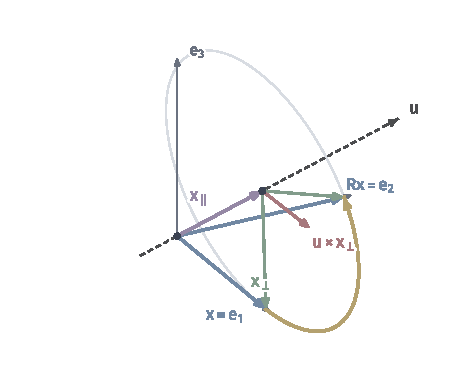
\includegraphics[width=80mm]{figures/04-spaces-measures-and-geometry/04-manifolds/matplotlib/lie-rodrigues-decomposition/figure.pdf}
  \caption{Rodrigues公式的分解。旋转轴$\bm u=(1,1,1)^\top/\sqrt3$，转角$2\pi/3$，$\bm x=\bm e_1$。紫色是沿轴分量$\bm x_\parallel$，保持不动；绿色是垂直分量$\bm x_\perp$，在灰色圆所在的平面内转动，转完后的绿色向量指向$\bm R\bm x$的末端；红色是$\bm u\times\bm x_\perp$的方向（长度按比例缩短）；黄色弧是端点走过的路径，终点是$\bm R\bm x=\bm e_2$。}
  \label{fig:lie-rodrigues-decomposition}
\end{BookInlineFigure}

\paragraph{每个旋转都有轴与角}
反过来，每个三维旋转都能写成式~\eqref{eq:lie-rodrigues}的形式，从而$\exp:\mathfrak{so}(3)\to\mathrm{SO}(3)$是满射。要证明这一点，先找出旋转的转轴，它是特征值$1$的特征向量，再看垂直于轴的平面。

\begin{theorem}[轴角表示]
\label{thm:lie-axis-angle}
对每个$\bm R\in\mathrm{SO}(3)$，存在单位向量$\bm u$与$\theta\in[0,\pi]$，使$\bm R=\exp(\theta[\bm u]_\times)$。并且
\begin{equation}
 \operatorname{tr}\bm R=1+2\cos\theta,\qquad \bm R-\bm R^\top=2\sin\theta\,[\bm u]_\times.
 \label{eq:lie-axis-angle-recovery}
\end{equation}
\end{theorem}

\begin{proof}
先找转轴。由$\bm R^\top\bm R=\bm I$与$\det\bm R=1$，得到
\[
\det(\bm R-\bm I)=\det\bigl(\bm R(\bm I-\bm R^\top)\bigr)
=\det(\bm I-\bm R^\top)=\det(\bm I-\bm R).
\]
三阶矩阵取负号使行列式变号，$\det(\bm I-\bm R)=-\det(\bm R-\bm I)$，于是$\det(\bm R-\bm I)=0$，存在单位向量$\bm u$使$\bm R\bm u=\bm u$。

再看与轴正交的平面。若$\bm x^\top\bm u=0$，则
\[
(\bm R\bm x)^\top\bm u=(\bm R\bm x)^\top(\bm R\bm u)=\bm x^\top\bm u=0,
\]
所以平面$\bm u^\perp$被$\bm R$映到自身。

取$\bm u^\perp$中的单位向量$\bm v$，令$\bm w=\bm u\times\bm v$，则$(\bm v,\bm w,\bm u)$是右手标准正交基。在这组基下$\bm R$的矩阵是分块对角的，左上二阶块正交，且行列式等于$\det\bm R=1$。由第~\ref{sec:lie-group-subgroup}节对$\mathrm{SO}(2)$的刻画，它等于某个$\bm R(\theta)$，$\theta\in[0,2\pi)$，即$\bm R\bm v=\cos\theta\,\bm v+\sin\theta\,\bm w$。

若$\theta\in(\pi,2\pi)$，把$\bm u$换成$-\bm u$、$\theta$换成$2\pi-\theta$，于是可取$\theta\in[0,\pi]$。这与定理~\ref{thm:lie-rodrigues}描述的作用在一组基上一致，所以二者相等。

最后，对式~\eqref{eq:lie-rodrigues}取迹。反对称矩阵的迹为零，并由式~\eqref{eq:lie-hat-square}，
\[
\operatorname{tr}[\bm u]_\times^2=\operatorname{tr}(\bm u\bm u^\top)-3=-2,
\]
于是
\[
\operatorname{tr}\bm R=3-2(1-\cos\theta)=1+2\cos\theta.
\]
减去转置时对称部分抵消，反对称部分加倍，得到第二式。
\end{proof}

这给出\term{轴角表示}（axis-angle representation），常把它合成一个向量$\bm\omega=\theta\bm u$，称为旋转向量。用式~\eqref{eq:lie-axis-angle-recovery}反算上面的循环轮换矩阵。它的迹为$0$，所以$\cos\theta=-\frac12$，$\theta=2\pi/3$。反对称部分给出
\[
\bm R-\bm R^\top=\begin{bmatrix}0&-1&1\\1&0&-1\\-1&1&0\end{bmatrix}
=2\sin\theta\,[\bm u]_\times,
\]
对照式~\eqref{eq:lie-hat-map}读出$\bm u\propto(1,1,1)^\top$，再由$2\sin\theta=\sqrt3$得到$\bm u=(1,1,1)^\top/\sqrt3$，回到了原来的轴和角。

\paragraph{冗余与特殊角度}
轴角表示有三类冗余。$(\bm u,\theta)$与$(-\bm u,-\theta)$给出同一旋转，$\theta$与$\theta+2\pi$也给出同一旋转，所以把$\theta$限制在$[0,\pi]$。在这个范围内，$0<\theta<\pi$时$\sin\theta>0$，式~\eqref{eq:lie-axis-angle-recovery}唯一地恢复$\theta$与$\bm u$。

剩下两个角度需要单独说明。$\theta=0$时$\bm R=\bm I$，任何轴都可以。$\theta=\pi$时$\bm R-\bm R^\top=\bm0$，轴$\bm u$与$-\bm u$给出同一旋转：绕一个轴转半圈，与绕相反的轴转半圈结果相同。

用旋转向量描述，映射$\bm\omega\mapsto\exp([\bm\omega]_\times)$把闭球$\{\lVert\bm\omega\rVert_2\leq\pi\}$映满$\mathrm{SO}(3)$；在开球$\lVert\bm\omega\rVert_2<\pi$内是单射，边界球面上互为相反数的两点给出同一个旋转。所以$\mathrm{SO}(3)$可以想象成一个实心球，球面上相对的点被粘合。

图~\ref{fig:lie-so3-ball}用这个模型画出绕$\bm e_3$的旋转：$\theta$从$0$增大到$\pi$时，$\bm\omega$沿半径走到$\pi\bm e_3$；继续增大，它从球面相对的一点$-\pi\bm e_3$重新进入，回到中心。这条路径在$\mathrm{SO}(3)$中是连续的闭合路径，并没有跳跃。

\begin{BookInlineFigure}
  \centering
  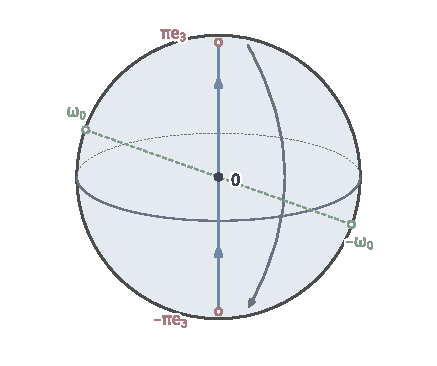
\includegraphics[width=74mm]{figures/04-spaces-measures-and-geometry/04-manifolds/matplotlib/lie-so3-ball/figure.pdf}
  \caption{$\mathrm{SO}(3)$的实心球模型。每个旋转向量$\bm\omega$的长度是转角，方向是转轴，闭球半径为$\pi$。边界上相对的两点（红圈$\pm\pi\bm e_3$，绿圈$\pm\bm\omega_0$）表示同一个旋转。蓝线是绕$\bm e_3$转一周的路径，走到$\pi\bm e_3$后，灰箭头表示它在$-\pi\bm e_3$处接着走，整条路径在$\mathrm{SO}(3)$中连续。}
  \label{fig:lie-so3-ball}
\end{BookInlineFigure}

在开球内，逆映射由式~\eqref{eq:lie-axis-angle-recovery}给出：
\[
\theta=\arccos\frac{\operatorname{tr}\bm R-1}{2},\qquad
[\bm\omega]_\times=\frac{\theta}{2\sin\theta}(\bm R-\bm R^\top),
\]
其中$\theta=0$处按极限$\theta/\sin\theta\to1$理解。所以旋转向量是$\mathrm{SO}(3)$去掉全部半圈旋转之后的局部坐标，与定理~\ref{thm:lie-so3-no-global-chart}一致：它不能延伸成全局坐标。

\paragraph{局部更新}
在一个已知旋转$\bm R$附近，常用$\bm R\exp([\bm\delta]_\times)$表示扰动后的旋转，其中$\bm\delta\in\mathbb R^3$很小。这是把单位元附近的指数坐标左平移到$\bm R$附近，参数$\bm\delta$在$\lVert\bm\delta\rVert_2<\pi$内与旋转一一对应。

一阶近似$\bm R+\bm R[\bm\delta]_\times$只是切空间中的一步，一般已不是正交矩阵；用指数代替它，结果严格留在$\mathrm{SO}(3)$中，这正是图~\ref{fig:lie-exp-limit}中折线与圆弧的区别。右乘$\exp([\bm\delta]_\times)$在物体自身的坐标系中扰动，左乘$\exp([\bm\delta]_\times)\bm R$则在固定的外部坐标系中扰动，二者一般不同，使用时须说明。

\paragraph{Euler角与万向节锁}
另一种常见的三参数记录是依次绕坐标轴旋转。记$\bm R_x,\bm R_y,\bm R_z$为绕三个坐标轴的旋转，取
\begin{equation}
 \bm R(\alpha,\beta,\gamma)=\bm R_z(\alpha)\bm R_y(\beta)\bm R_x(\gamma),
 \label{eq:lie-euler-angles}
\end{equation}
三个角称为一组\term{Euler角}（Euler angles）。它便于解释，却在特殊角度失去局部坐标的作用，原因在于三个参数对应的瞬时转轴可能共线。

把式~\eqref{eq:lie-euler-angles}分别对三个角求导，再右乘$\bm R^\top$，得到每个参数产生的角速度方向。用$\bm R_z(\alpha)$与$\bm R_y(\beta)$共轭后，三个方向是
\[
\bm a_\alpha=\bm e_3,\qquad
\bm a_\beta=\bm R_z(\alpha)\bm e_2,\qquad
\bm a_\gamma=\bm R_z(\alpha)\bm R_y(\beta)\bm e_1 .
\]
以$\bm a_\gamma$为例，把$\bm R_x$的导数写成$\bm R_x[\bm e_1]_\times$（绕$\bm e_1$转动的方向），再把两侧的转动并进叉积，得到
\[
\partial_\gamma\bm R\,\bm R^\top
=\bm R_z\bm R_y[\bm e_1]_\times\bm R_y^\top\bm R_z^\top
=[\bm R_z\bm R_y\bm e_1]_\times .
\]

这三个方向的线性无关性决定了参数化是否满秩。由
\[
\bm R_y(\beta)\bm e_1=(\cos\beta,0,-\sin\beta)^\top,
\]
并把三个向量都乘以$\bm R_z(\alpha)^\top$（不改变行列式），得到
\[
\det[\bm a_\alpha,\bm a_\beta,\bm a_\gamma]
=\det\begin{bmatrix}0&0&\cos\beta\\0&1&0\\1&0&-\sin\beta\end{bmatrix}
=-\cos\beta .
\]
当$\beta=\pm\pi/2$时行列式为零，参数到旋转的微分秩降为$2$。

\begin{BookInlineFigure}
  \centering
  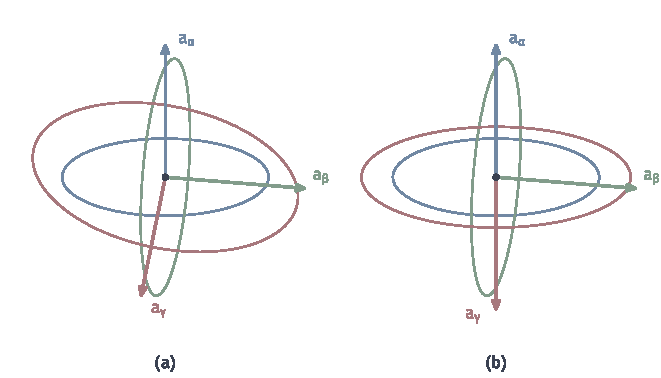
\includegraphics[width=112mm]{figures/04-spaces-measures-and-geometry/04-manifolds/matplotlib/lie-gimbal-lock/figure.pdf}
  \caption{Euler角的三个瞬时转轴。蓝、绿、红箭头分别是$\alpha,\beta,\gamma$对应的转轴$\bm a_\alpha,\bm a_\beta,\bm a_\gamma$，同色圆环垂直于该轴（这里$\alpha=20^\circ$）。(a)$\beta=35^\circ$，三根轴线性无关，任何方向的小转动都能实现。(b)$\beta=90^\circ$，$\bm a_\gamma=-\bm e_3$与$\bm a_\alpha$共线，两个圆环重合在同一平面内，只剩两个独立的转动方向。}
  \label{fig:lie-gimbal-lock}
\end{BookInlineFigure}

直接代入也能看到这一点。由$\bm R_y(\pi/2)\bm e_1=-\bm e_3$，绕$\bm e_1$的旋转经$\bm R_y(\pi/2)$共轭后变为绕$-\bm e_3$的旋转，即
\[
\bm R_y(\tfrac\pi2)\bm R_x(\gamma)=\bm R_z(-\gamma)\bm R_y(\tfrac\pi2).
\]
于是
\[
\bm R(\alpha,\tfrac\pi2,\gamma)=\bm R_z(\alpha-\gamma)\bm R_y(\tfrac\pi2).
\]
结果只依赖$\alpha-\gamma$：同时把$\alpha,\gamma$加上同一个数，旋转不变。这称为\term{万向节锁}（gimbal lock），图~\ref{fig:lie-gimbal-lock}(b)中蓝、红两根轴共线正是它的几何原因。

万向节锁是坐标的奇异，不是旋转本身的退化。$\bm R(\alpha,\pi/2,\gamma)$仍是合法的旋转，$\mathrm{SO}(3)$在它附近仍是三维流形；只是这一组角在该处不能作为坐标，附近的小转动也可能要求角度大幅跳动。换一种轴的次序或改用旋转向量，就能在这里重新得到正常的局部坐标。

\subsection{单位四元数}
\label{sec:lie-unit-quaternions}

旋转矩阵用九个数，轴角在半圈处与恒等处需要特别处理。单位四元数用四个数和一个单位长度约束记录旋转，复合只需一次乘法，并且在每一点附近都给出正常的局部坐标，代价是每个旋转恰有两个记录。

\paragraph{四元数及其运算}
把\term{四元数}（quaternion）写成标量部与三维向量部组成的对$q=(s,\bm u)$，其中$s\in\mathbb R$、$\bm u\in\mathbb R^3$。加法与数乘按$\mathbb R^4$进行，乘法规定为
\begin{equation}
 (s,\bm u)(t,\bm v)=(st-\bm u^\top\bm v,\ s\bm v+t\bm u+\bm u\times\bm v).
 \label{eq:lie-quaternion-product}
\end{equation}
类比复数：标量部相当于实部，向量部相当于“虚部”，只是虚部有三个方向，它们之间的乘法由叉积描述。

因为含有叉积，乘法一般不交换：$(0,\bm e_1)(0,\bm e_2)=(0,\bm e_3)$，而$(0,\bm e_2)(0,\bm e_1)=(0,-\bm e_3)$。$(1,\bm0)$是乘法单位元。乘法满足结合律，把三重乘积按式~\eqref{eq:lie-quaternion-product}展开，用二重叉积公式整理即可验证，这里略去这段机械的展开。

共轭定义为$q^*=(s,-\bm u)$，范数定义为$\lvert q\rvert=\sqrt{s^2+\lVert\bm u\rVert_2^2}$，即$\mathbb R^4$中的欧氏长度。由式~\eqref{eq:lie-quaternion-product}，
\[
qq^*=\bigl(s^2+\bm u^\top\bm u,\ -s\bm u+s\bm u-\bm u\times\bm u\bigr)
=(\lvert q\rvert^2,\bm0),
\]
同理$q^*q=(\lvert q\rvert^2,\bm0)$。直接展开还可验证$(pq)^*=q^*p^*$。

下面的引理说明范数与乘法相容，这是四元数能表示旋转的基础。

\begin{lemma}[范数的乘法性]
\label{lem:lie-quaternion-norm}
对四元数$p,q$，$\lvert pq\rvert=\lvert p\rvert\,\lvert q\rvert$。因此$\lvert q\rvert=1$的\term{单位四元数}（unit quaternion）在乘法下构成群，$q^{-1}=q^*$；作为集合，它就是$\mathbb R^4$中的单位球面$S^3$。
\end{lemma}

\begin{proof}
设$p=(s,\bm u)$、$q=(t,\bm v)$。向量部$s\bm v+t\bm u+\bm u\times\bm v$中，$\bm u\times\bm v$与$\bm u,\bm v$都正交，所以
\[
\lvert pq\rvert^2=(st-\bm u^\top\bm v)^2+\lVert s\bm v+t\bm u\rVert_2^2+\lVert\bm u\times\bm v\rVert_2^2.
\]
展开平方后，交叉项$-2st\,\bm u^\top\bm v$与$+2st\,\bm u^\top\bm v$相消，剩下
\[
s^2t^2+s^2\lVert\bm v\rVert_2^2+t^2\lVert\bm u\rVert_2^2+(\bm u^\top\bm v)^2+\lVert\bm u\times\bm v\rVert_2^2.
\]
由Lagrange恒等式
\[
(\bm u^\top\bm v)^2+\lVert\bm u\times\bm v\rVert_2^2=\lVert\bm u\rVert_2^2\lVert\bm v\rVert_2^2,
\]
上式等于
\[
(s^2+\lVert\bm u\rVert_2^2)(t^2+\lVert\bm v\rVert_2^2).
\]
于是单位四元数的乘积仍是单位四元数，$qq^*=(1,\bm0)$给出逆元，结合律继承自全体四元数。
\end{proof}

\paragraph{用共轭作用表示旋转}
把向量$\bm x$嵌入为向量部，即纯四元数$(0,\bm x)$。对单位四元数$q=(s,\bm u)$，分两步计算$q(0,\bm x)q^*$。先由式~\eqref{eq:lie-quaternion-product}左乘，得到
\[
q(0,\bm x)=(-\bm u^\top\bm x,\ s\bm x+\bm u\times\bm x).
\]

再右乘$q^*=(s,-\bm u)$。标量部是
\[
(-\bm u^\top\bm x)s+(s\bm x+\bm u\times\bm x)^\top\bm u=0,
\]
这是因为$\bm u\times\bm x$与$\bm u$正交。向量部用二重叉积公式
\[
(\bm u\times\bm x)\times\bm u=\lVert\bm u\rVert_2^2\bm x-(\bm u^\top\bm x)\bm u
\]
整理，得到
\begin{equation}
 \begin{gathered}
 q(0,\bm x)q^*=(0,\bm R(q)\bm x),\\
 \bm R(q)\bm x=(s^2-\lVert\bm u\rVert_2^2)\bm x+2\bm u(\bm u^\top\bm x)+2s\,\bm u\times\bm x.
 \end{gathered}
 \label{eq:lie-quaternion-rotation}
\end{equation}

取$q=(\cos\frac\theta2,\ \sin\frac\theta2\,\bm a)$，其中$\lVert\bm a\rVert_2=1$。由半角公式，
\[
s^2-\lVert\bm u\rVert_2^2=\cos\theta,\qquad
2\bm u\bm u^\top=(1-\cos\theta)\bm a\bm a^\top,\qquad
2s\bm u=\sin\theta\,\bm a.
\]
代入式~\eqref{eq:lie-quaternion-rotation}，再用式~\eqref{eq:lie-hat-square}，得到
\[
\begin{aligned}
\bm R(q)
&=\cos\theta\,\bm I+(1-\cos\theta)\bm a\bm a^\top+\sin\theta\,[\bm a]_\times\\
&=\bm I+\sin\theta\,[\bm a]_\times+(1-\cos\theta)[\bm a]_\times^2 .
\end{aligned}
\]
这正是Rodrigues公式~\eqref{eq:lie-rodrigues}：$q$表示绕$\bm a$转角$\theta$。半角来自$q$在两侧各乘一次，不是把物理转角减半。

\paragraph{复合与双覆盖}
手算两个旋转的复合。设$q_1=(\frac{\sqrt2}2,\ \frac{\sqrt2}2\bm e_3)$表示绕$\bm e_3$转$90^\circ$，$q_2=(\frac{\sqrt2}2,\ \frac{\sqrt2}2\bm e_1)$表示绕$\bm e_1$转$90^\circ$，先做$q_1$、再做$q_2$。由式~\eqref{eq:lie-quaternion-product}，
\[
q_2q_1=\Bigl(\tfrac12,\ \tfrac12\bm e_3+\tfrac12\bm e_1+\tfrac12\bm e_1\times\bm e_3\Bigr)
=\Bigl(\tfrac12,\ \tfrac12(1,-1,1)^\top\Bigr).
\]

读出半角：$\cos\frac\theta2=\frac12$，所以$\theta=2\pi/3$，转轴是$(1,-1,1)^\top/\sqrt3$。用式~\eqref{eq:lie-quaternion-rotation}计算$\bm e_1$的像，三项分别是$-\frac12\bm e_1$、$\frac12(1,-1,1)^\top$、$\frac12(0,1,1)^\top$，相加得到$\bm e_3$。

直接用矩阵核对，
\[
\bm R_x(\tfrac\pi2)\bm R_z(\tfrac\pi2)\bm e_1=\bm R_x(\tfrac\pi2)\bm e_2=\bm e_3 ,
\]
结果一致。复合用四元数只需一次乘法，读出轴和角也只需看四个数。

这个计算说明的是一般事实。由结合律与$(q_2q_1)^*=q_1^*q_2^*$，
\[
(q_2q_1)(0,\bm x)(q_2q_1)^*=q_2\bigl(q_1(0,\bm x)q_1^*\bigr)q_2^* ,
\]
即$\bm R(q_2q_1)=\bm R(q_2)\bm R(q_1)$。所以$q\mapsto\bm R(q)$是从单位四元数群到$\mathrm{SO}(3)$的群同态。由定理~\ref{thm:lie-axis-angle}，每个旋转都有轴与角，从而有形如上式的四元数，这个同态是满射。它的核由下面的定理确定。

\begin{theorem}[单位四元数的双覆盖]
\label{thm:lie-double-cover}
对单位四元数$q_1,q_2$，$\bm R(q_1)=\bm R(q_2)$当且仅当$q_2=\pm q_1$。
\end{theorem}

\begin{proof}
由定理~\ref{thm:lie-kernel-injective}，只需证明核为$\{(1,\bm0),(-1,\bm0)\}$。设$q=(s,\bm u)$是单位四元数，$\bm R(q)=\bm I$。

若$\bm u\neq\bm0$，取与$\bm u$正交的非零向量$\bm x$。由式~\eqref{eq:lie-quaternion-rotation}与$s^2+\lVert\bm u\rVert_2^2=1$，$\bm x=\bm R(q)\bm x$成为
\[
\bm x=(1-2\lVert\bm u\rVert_2^2)\bm x+2s\,\bm u\times\bm x,
\]
移项得到
\[
-2\lVert\bm u\rVert_2^2\bm x+2s\,\bm u\times\bm x=\bm0 .
\]
两项分别与$\bm x$平行、与$\bm x$正交，必须各为零，第一项非零，矛盾。

所以$\bm u=\bm0$，由单位长度得$s=\pm1$。反过来，$\pm(1,\bm0)$代入式~\eqref{eq:lie-quaternion-rotation}给出$\bm I$。
\end{proof}

这称为单位四元数对$\mathrm{SO}(3)$的\term{双覆盖}（double cover）：每个旋转恰有两个单位四元数，二者互为相反数。上面的$q_1$与$-q_1=(-\frac{\sqrt2}2,-\frac{\sqrt2}2\bm e_3)$表示同一个旋转，后者对应转角$\pi/2+2\pi$的半角。图~\ref{fig:lie-double-cover}把$S^3$限制到一条大圆上画出这个现象。

\begin{BookInlineFigure}
  \centering
  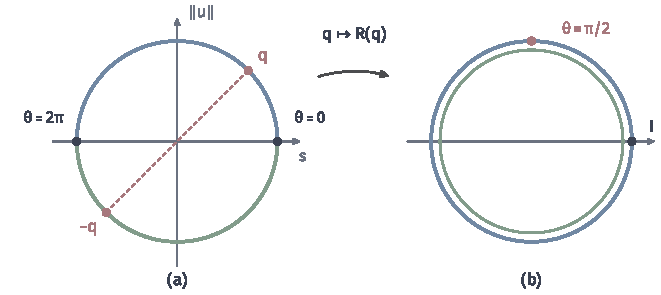
\includegraphics[width=112mm]{figures/04-spaces-measures-and-geometry/04-manifolds/matplotlib/lie-double-cover/figure.pdf}
  \caption{半角与双覆盖。固定转轴$\bm a$，单位四元数$(\cos\frac\theta2,\sin\frac\theta2\,\bm a)$在$S^3$中走出一条大圆。(a)这条大圆，横轴为标量部，纵轴为沿$\bm a$的向量部。$\theta$从$0$到$2\pi$时走过蓝色半圆，从$2\pi$到$4\pi$时走过绿色半圆，$q$与$-q$（红点）相对。(b)绕$\bm a$的旋转组成的圆，$\theta$走一周即回到$\bm I$，蓝、绿两个半圆分别映满整个圆，$q$与$-q$映到同一点。}
  \label{fig:lie-double-cover}
\end{BookInlineFigure}

双覆盖与坐标奇异是两回事。$q\mapsto\bm R(q)$在每一点都是局部微分同胚。在$q=(1,\bm0)$附近，
\[
\bm R(q)=\bm I+2[\bm u]_\times+O(\lVert\bm u\rVert_2^2),
\]
微分$\bm u\mapsto2[\bm u]_\times$是从切空间$T_{(1,\bm0)}S^3=\{(0,\bm u)\}$到$\mathfrak{so}(3)$的线性同构；在其他点用群乘法平移即得。

所以单位四元数在任何朝向附近都给出正常的局部坐标，不会出现Euler角那样的秩下降。$q$与$-q$之差也不是额外的物理自由度：$S^3$与$\mathrm{SO}(3)$都是三维，符号只是整体上的二选一。

\paragraph{计算中的注意事项}
按式~\eqref{eq:lie-quaternion-product}，两个四元数相乘需要$16$次实数乘法，两个三阶矩阵相乘需要$27$次。数值计算中多次相乘会使$\lvert q\rvert$逐渐偏离$1$；若$\lvert q\rvert\neq1$，$q(0,\bm x)q^*$会额外把$\bm x$放大$\lvert q\rvert^2$倍，不再是旋转，所以需要定期把$q$除以$\lvert q\rvert$。

比较两个四元数是否接近时，还要考虑符号：$q$与$-q$在$\mathbb R^4$中相距$2$，表示的却是同一个旋转。表~\ref{tab:lie-rotation-representations}汇总了本节比较的各种表示。

\begin{BookInlineTable}
  \centering
  \caption{三维旋转的几种表示}
  \label{tab:lie-rotation-representations}
  \begin{tabular}{lll}
    \toprule
    表示 & 参数与约束 & 冗余或奇异 \\
    \midrule
    旋转矩阵 & $9$个数，$6$个约束 & 无冗余，运算需保持约束 \\
    轴角 & $3$个数，$\lVert\bm\omega\rVert_2\leq\pi$ & 半圈处$\pm\bm\omega$相同 \\
    Euler角 & $3$个数 & $\beta=\pm\pi/2$处秩降为$2$ \\
    单位四元数 & $4$个数，$1$个约束 & $q$与$-q$相同，无奇异 \\
    \bottomrule
  \end{tabular}
\end{BookInlineTable}

\section{刚体位姿}
\label{sec:lie-rigid-poses}

一个刚体在空间中的状态由两部分决定：它朝向哪里，以及它的参考点在哪里。前者是上一节的旋转，后者是一个平移。可以证明，保持任意两点距离与空间定向的变换恰好是先旋转、再平移的复合（这里不给出证明）；这样的变换称为\term{刚体变换}（rigid transformation），它描述的状态称为\term{位姿}（pose）。本节建立刚体变换的复合与求逆，说明它在点与方向上的不同作用，最后用它表达坐标系之间的换算。

\paragraph{齐次矩阵}
刚体变换把$\bm x$变成$\bm R\bm x+\bm t$，其中$\bm R\in\mathrm{SO}(3)$、$\bm t\in\mathbb R^3$。它不是线性映射，因为原点被移到$\bm t$。在每个点后面补一个坐标$1$，就能把它写成一次矩阵乘法：
\begin{equation}
 \begin{bmatrix}\bm R\bm x+\bm t\\1\end{bmatrix}=\bm T\begin{bmatrix}\bm x\\1\end{bmatrix},\qquad
 \bm T=\begin{bmatrix}\bm R&\bm t\\\bm0^\top&1\end{bmatrix}.
 \label{eq:lie-homogeneous-pose}
\end{equation}
这样的$4\times4$矩阵全体记为$\mathrm{SE}(3)$，称为\term{三维刚体运动群}（three-dimensional rigid-motion group）。

\paragraph{复合与求逆}
按分块乘法，先作用$\bm T_1$、再作用$\bm T_2$得到
\begin{equation}
 \bm T_2\bm T_1=\begin{bmatrix}\bm R_2\bm R_1&\bm R_2\bm t_1+\bm t_2\\\bm0^\top&1\end{bmatrix},\qquad
 \bm T^{-1}=\begin{bmatrix}\bm R^\top&-\bm R^\top\bm t\\\bm0^\top&1\end{bmatrix}.
 \label{eq:lie-pose-composition}
\end{equation}
乘积仍是同样形状的矩阵，逆矩阵也是，单位元是$\bm I_4$，所以$\mathrm{SE}(3)$是$\mathrm{GL}(4,\mathbb R)$的子群。求逆的公式可以直接解出：由$\bm y=\bm R\bm x+\bm t$得$\bm x=\bm R^\top(\bm y-\bm t)=\bm R^\top\bm y-\bm R^\top\bm t$。

复合的平移部分是$\bm R_2\bm t_1+\bm t_2$，而不是$\bm t_1+\bm t_2$：第一次的平移要随第二次的旋转一起转动。例如两次都绕$\bm e_3$转$\pi/2$，平移分别为$\bm t_1=(1,0,0)^\top$与$\bm t_2=(0,1,0)^\top$。复合的旋转是绕$\bm e_3$转$\pi$，平移是$\bm R_2\bm t_1+\bm t_2=(0,1,0)^\top+(0,1,0)^\top=(0,2,0)^\top$。按另一次序复合，平移变成$\bm R_1\bm t_2+\bm t_1=(-1,0,0)^\top+(1,0,0)^\top=\bm0$，结果不同。

\paragraph{作为Lie群}
$\mathrm{SE}(3)$在$\mathrm{GL}(4,\mathbb R)$中由“左上块在$\mathrm{SO}(3)$中、末行为$(0,0,0,1)$”这些闭条件给出，是闭子群，因而是矩阵Lie群。$(\bm R,\bm t)\mapsto\bm T$是从$\mathrm{SO}(3)\times\mathbb R^3$到$\mathrm{SE}(3)$的微分同胚，所以$\mathrm{SE}(3)$是六维流形：三个旋转自由度加三个平移自由度。但作为群，它不是$\mathrm{SO}(3)$与$\mathbb R^3$的直积：直积的运算会给出$(\bm R_2\bm R_1,\bm t_1+\bm t_2)$，而式~\eqref{eq:lie-pose-composition}中旋转会作用到前一次的平移上。

对经过$\bm I_4$的曲线求导，末行恒为零、左上块的导数在$\mathfrak{so}(3)$中，所以Lie代数是
\[
\mathfrak{se}(3)=\left\{\begin{bmatrix}[\bm\omega]_\times&\bm v\\\bm0^\top&0\end{bmatrix}:\bm\omega,\bm v\in\mathbb R^3\right\}.
\]
用归纳法可得，对$k\geq1$，该矩阵的$k$次幂是$\begin{bmatrix}[\bm\omega]_\times^k&[\bm\omega]_\times^{k-1}\bm v\\\bm0^\top&0\end{bmatrix}$，于是
\[
\exp\begin{bmatrix}[\bm\omega]_\times&\bm v\\\bm0^\top&0\end{bmatrix}
=\begin{bmatrix}\exp([\bm\omega]_\times)&\bm V\bm v\\\bm0^\top&1\end{bmatrix},\qquad
\bm V=\sum_{k\geq0}\frac{[\bm\omega]_\times^k}{(k+1)!}.
\]
$\bm\omega=\bm0$时$\bm V=\bm I$，指数就是平移$\bm v$；$\bm\omega\neq\bm0$时，平移部分是$\bm V\bm v$而不是$\bm v$，单参数子群一般绕某条轴转动、同时沿该轴推进（推进量可以为零），是一种螺旋运动。所以$\mathrm{SE}(3)$上的指数坐标不等于“旋转向量加平移向量”这种分开的记录，使用时须说明采用哪一种参数化。

\paragraph{点与方向}
位姿对点和方向的作用不同。点有位置，平移会移动它；方向只有朝向，例如速度、表面法向或两点之差，平移不应改变它。设$\bm x,\bm y$是两个点，它们的差在变换后为$(\bm R\bm x+\bm t)-(\bm R\bm y+\bm t)=\bm R(\bm x-\bm y)$，平移抵消了。在齐次写法中，把点记为$(\bm x,1)$，把方向记为$(\bm d,0)$，则
\[
\bm T\begin{bmatrix}\bm d\\0\end{bmatrix}=\begin{bmatrix}\bm R\bm d\\0\end{bmatrix},
\]
末坐标$0$恰好让平移列不起作用，两个点之差的末坐标也自然是$1-1=0$。

点与方向的区分在计算中容易出错。把方向向量当成点，用$\bm R\bm d+\bm t$变换，会给方向加上一个与位姿有关的偏移；把点当成方向，则会丢掉平移。若变换是一般的可逆线性映射$\bm A$而不是旋转，法向量要按$\bm A^{-\top}$变换才能保持与切向量的正交；对旋转，$\bm R^{-\top}=\bm R$，法向与其他方向按同一规则变换。

\paragraph{坐标系变换}
同一个点在不同坐标系中有不同的坐标，刚体变换也负责这种换算。设坐标系$B$的原点在坐标系$A$中的坐标为$\bm t_{AB}$，$B$的三个坐标轴在$A$中的方向依次是$\bm R_{AB}$的三列。若一点在$B$中的坐标为$\bm x_B$，它在$A$中的位置是$B$的原点加上沿$B$各轴的位移，即
\[
\bm x_A=\bm R_{AB}\bm x_B+\bm t_{AB},\qquad
\bm T_{AB}=\begin{bmatrix}\bm R_{AB}&\bm t_{AB}\\\bm0^\top&1\end{bmatrix}.
\]
这里$\bm T_{AB}$读作“从$B$的坐标到$A$的坐标”。由此得到两条规则：经过中间坐标系$B$换算，$\bm T_{AC}=\bm T_{AB}\bm T_{BC}$，相邻下标相同才能相乘；反向换算是求逆，$\bm T_{BA}=\bm T_{AB}^{-1}$。

同一个矩阵$\bm T_{AB}$有两种读法：它可以看作把点从一个位置移到另一个位置的主动变换，也可以看作同一个点在两个坐标系之间的坐标换算。两种读法使用同一套矩阵运算，但描述的对象不同；混淆二者，最常见的后果是该用$\bm T$的地方用了$\bm T^{-1}$，或者乘积次序颠倒。

给定一组点在两个坐标系中的对应坐标，要反求$\bm R_{AB}$与$\bm t_{AB}$，这就是由点对应估计刚体变换的问题。它需要拟合目标、正交约束下的求解与可辨识性分析，在第~\ref{chap:spatial-map-estimation}章研究。

\section{商流形}
\label{sec:lie-quotients}

前面几节反复遇到“多种记录代表同一对象”：$q$与$-q$表示同一个旋转；图~\ref{fig:lie-sphere-cosets}中一整圈旋转把$\bm e_3$送到同一个点；一个观测只确定方向时，$(2,1)^\top$与$(4,2)^\top$应视为同一对象；同一个子空间可以用许多组基张成。这些冗余都来自一个群作用：它作用在记录上，而不改变所表示的对象。把同一轨道中的记录合并，就得到真正要研究的对象集合。

第~\ref{chap:topological-spaces}章为等价关系的商集合规定了商拓扑：设$q:M\to M/G$把每个点送到所在的轨道，商中的子集$U$为开集，当且仅当$q^{-1}(U)$在$M$中为开集。本节要进一步回答：什么时候这个商还能带上光滑结构，使后面几章的切空间、微分与度量都能使用。任意群作用的商一般做不到这一点。

\subsection{光滑商的条件}
\label{sec:lie-smooth-quotient-conditions}

先看两个商不是流形的例子，从中读出群作用需要满足的条件，再陈述这些条件下的商流形定理，并用闭子群构造最常用的一类商。

\paragraph{两类失败}
第一类失败来自稳定子不一致。第~\ref{sec:lie-orbits-stabilizers}节中，$\mathrm{SO}(2)$作用于$\mathbb R^2$的商是$[0,\infty)$。非零点的轨道是圆，稳定子平凡；原点的轨道是一个点，稳定子是整个群。商在$0$处有一个端点，那里的任何邻域都不同胚于开区间，所以商不是无边界的一维流形，见图~\ref{fig:lie-quotient-failures}(a)(b)。不能只因为“去掉了一个旋转自由度”就宣布商是$2-1=1$维流形。

第二类失败来自轨道挤在一起。取无理数$\alpha$，让整数加法群$\mathbb Z$按$k\cdot\bm x=\bm R(2\pi k\alpha)\bm x$作用在单位圆上。$k\neq0$时$k\alpha$不是整数，没有点被固定，稳定子都是平凡的。但每条轨道都在圆上稠密。

下面证明这一点。把圆分成$N$段长为$2\pi/N$的弧，同一条轨道上$k=0,1,\ldots,N$这$N+1$个点必有两个落在同一段，设为$k_1<k_2$。令$k=k_2-k_1$，则转角$2\pi k\alpha$模$2\pi$后绝对值小于$2\pi/N$，且不为零。反复施加这个小旋转，轨道上就出现间距小于$2\pi/N$的点，$N$可以任意大，所以轨道稠密。

\begin{BookInlineFigure}
  \centering
  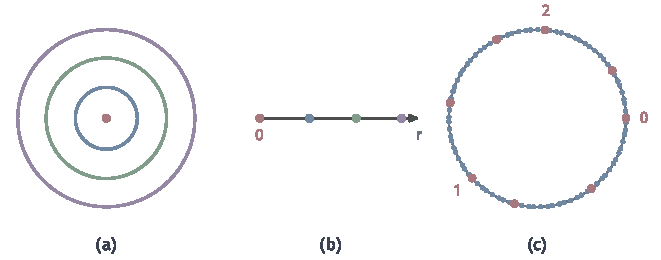
\includegraphics[width=112mm]{figures/04-spaces-measures-and-geometry/04-manifolds/matplotlib/lie-quotient-failures/figure.pdf}
  \caption{商不是流形的两种情形。(a)$\mathrm{SO}(2)$作用于平面的轨道：同心圆与中心的原点。(b)轨道空间$[0,\infty)$，用半径编号，同色的点对应同色的圆，原点（红）对应端点。(c)无理旋转的一条轨道，$\alpha=(\sqrt5-1)/2$，大红点依次是前$8$个点$k=0,\ldots,7$，小蓝点是$k=8,\ldots,89$，已经密布整个圆。}
  \label{fig:lie-quotient-failures}
\end{BookInlineFigure}

于是商空间的拓扑很差。设$U$是商中的非空开集，它的原像是圆上的非空开集，且由整条轨道组成。任何一条轨道都稠密，所以都与这个开集相交，从而整条轨道都在其中，$U$就是整个商。商的开集只有空集和全集，不同的点不能被开集分开，它不是Hausdorff空间，更不是流形。

\paragraph{自由与适当}
这两类失败分别对应下面两个条件。

\begin{definition}[自由作用与适当作用]
\label{def:lie-free-proper-action}
设Lie群$G$光滑地作用于流形$M$，即$G\times M\to M$是光滑映射。若每个点的稳定子都只含单位元，就称作用是\term{自由作用}（free action）。若映射$G\times M\to M\times M$，$(g,x)\mapsto(g\cdot x,x)$下每个紧集的原像都是紧集，就称作用是\term{适当作用}（proper action）。
\end{definition}

自由性排除了第一类失败：各点的稳定子相同，轨道的维数处处等于群的维数。适当性排除了第二类失败：它禁止群中“跑到无穷远”的元素把一个点又带回原处附近，从而使不同的轨道能被邻域分开。

紧Lie群的光滑作用总是适当的，有限群作为零维Lie群也是如此。上面的$\mathbb Z$作用不适当：取$\bm x$的一个邻域，无穷多个$k$把$\bm x$送回这个邻域，这些$k$组成无界的集合。下面的定理说明，这两个条件足以得到光滑的商。

\begin{theorem}[商流形定理]
\label{thm:lie-quotient-manifold}
设Lie群$G$在$m$维光滑流形$M$上的光滑作用既自由又适当，$G$的维数为$k$。则轨道空间$M/G$在商拓扑下是$m-k$维的拓扑流形，并且具有唯一的光滑结构，使商映射$q:M\to M/G$是光滑淹没。
\end{theorem}

定理的证明需要构造横截于轨道的局部切片，并用常秩定理验证转移映射光滑，篇幅较长，读者可查阅\scite{math-lee2013smooth}。证明的思路是：在每个点附近，取与轨道横截的一小片子流形，由自由与适当两个条件，每条附近的轨道与这片子流形恰好相交一次，这片子流形就充当商的坐标图。

所得的光滑结构称为\term{商流形}（quotient manifold）。由$q$是淹没，$M/G$上的映射$f$光滑，当且仅当$f\circ q$在$M$上光滑。第~\ref{sec:lie-invariant-equivariant}节中经由轨道分解的不变映射，正是用这种方式落到商上。

定理给的是充分条件，不是唯一可用的情形。对没有给定作用的一般等价关系，商可能根本不是流形；即使作用存在，也要逐项核对光滑、自由与适当，不能把任意等价关系的商都当作光滑流形。

\paragraph{齐性空间}
最常用的一类商来自闭子群。设$H$是Lie群$G$的闭子群，它按$h\cdot g=gh^{-1}$作用在$G$上，轨道恰是左陪集$gH$。这个作用自由，并且可以证明是适当的（闭性保证陪集不会挤在一起），所以$G/H$是$\dim G-\dim H$维的流形，称为\term{齐性空间}（homogeneous space）。它之所以“齐性”，是因为$G$按$g'\cdot(gH)=(g'g)H$传递地作用在$G/H$上，任何两点之间都有一个变换相连。

齐性空间常常就是某个熟悉的空间。若$G$光滑且传递地作用于流形$X$，$x_0\in X$的稳定子为$H$，由定理~\ref{thm:lie-orbit-stabilizer}，$gH\mapsto g\cdot x_0$是从$G/H$到$X$的双射，并且可以进一步证明它是微分同胚。以$\mathrm{SO}(3)$作用于$S^2$为例，$\bm e_3$的稳定子是绕第三轴的旋转，与$\mathrm{SO}(2)$同构，所以
\begin{equation}
 \mathrm{SO}(3)/\mathrm{SO}(2)\cong S^2,\qquad \bm R\,\mathrm{SO}(2)\mapsto\bm R\bm e_3.
 \label{eq:lie-so3-so2}
\end{equation}

维数核对：$3-1=2$。图~\ref{fig:lie-sphere-cosets}(b)画的正是这个商的一条纤维：$\bm R$的第三列决定了陪集，前两列在切平面内还可以任意转动，这一转动正是被商掉的自由度。

另一个例子回到四元数。有限群$\{(1,\bm0),(-1,\bm0)\}$按左乘作用在$S^3$上，没有不动点，作用自由且适当，商$S^3/\{\pm1\}$是三维流形。由定理~\ref{thm:lie-double-cover}，$q\mapsto\bm R(q)$在每条轨道$\{q,-q\}$上取同一个值，并且不同的轨道给出不同的旋转，于是它在商上给出$S^3/\{\pm1\}$到$\mathrm{SO}(3)$的双射；结合它是局部微分同胚，可知这个双射是微分同胚。

\subsection{射影空间}
\label{sec:lie-projective-space}

相机把空间中的一点投影到成像平面时，只能确定这一点所在的视线方向，不能确定它沿视线有多远。若把视线用一个非零向量记录，那么$\bm x$与$\lambda\bm x$（$\lambda\neq0$）记录的是同一条视线。忽略这种非零倍数，就得到射影空间。

\begin{definition}[实射影空间]
\label{def:lie-projective-space}
非零实数在乘法下构成群$\mathbb R^*=\mathbb R\setminus\{0\}$，它按$\lambda\cdot\bm x=\lambda\bm x$作用于$\mathbb R^{n+1}\setminus\{\bm0\}$。轨道空间
\begin{equation}
 \mathbb{RP}^n=(\mathbb R^{n+1}\setminus\{\bm0\})/\mathbb R^*
 \label{eq:lie-rpn}
\end{equation}
称为$n$维\term{实射影空间}（real projective space）。$\bm x$所在的轨道记为$[\bm x]=[x_1:\cdots:x_{n+1}]$，称为\term{齐次坐标}（homogeneous coordinates）。
\end{definition}

$\mathbb{RP}^n$的一个点就是$\mathbb R^{n+1}$中过原点的一条直线。零向量必须除去：它的所有倍数都是零，不表示任何方向。这个作用是自由的，因为$\lambda\bm x=\bm x$与$\bm x\neq\bm0$推出$\lambda=1$。

作用也是适当的。设$K$是$(\mathbb R^{n+1}\setminus\{\bm0\})^2$中的紧集，$K$的两个分量的范数都落在某个区间$[a,b]$内，$a>0$。若$(\lambda\bm x,\bm x)\in K$，则
\[
\lvert\lambda\rvert=\frac{\lVert\lambda\bm x\rVert_2}{\lVert\bm x\rVert_2}\in\Bigl[\frac ab,\frac ba\Bigr].
\]
所以原像中的$\lambda$在$\mathbb R^*$的紧子集内，$\bm x$在$K$的投影内，原像又是闭集，从而是紧集。由定理~\ref{thm:lie-quotient-manifold}，$\mathbb{RP}^n$是$n$维光滑流形，维数核对$(n+1)-1=n$。把代表元缩放到单位球面，只剩符号自由度，于是它也可以写成$S^n/\{\pm1\}$。

\paragraph{仿射图与无穷远点}
商流形的坐标可以直接写出来。在$x_j\neq0$的点上，每个类都唯一地有一个代表使第$j$个分量为$1$，于是令
\[
U_j=\{[\bm x]:x_j\neq0\},\qquad
\varphi_j([\bm x])=\Bigl(\frac{x_i}{x_j}\Bigr)_{i\neq j}\in\mathbb R^n .
\]
$\varphi_j$不依赖代表元，因为分子分母同乘$\lambda$。$U_j$的原像$\{x_j\neq0\}$是开集，所以$U_j$是开集。$\varphi_j\circ q$是有理函数，因而连续；逆映射把$\bm u$送到第$j$分量为$1$的向量再取类，也连续，所以$\varphi_j$是同胚。两张图的重叠处，坐标转换是分量之比，分母非零，因而光滑。这些图称为\term{仿射图}（affine chart），$n+1$张就覆盖了$\mathbb{RP}^n$。

相对于一张选定的仿射图$U_{n+1}$，不在其中的点$\{x_{n+1}=0\}$称为\term{无穷远点}（point at infinity）。它们不是向坐标中加入数值$\infty$，而是这张图未覆盖、在其他图中可以正常记录的点。

看$\mathbb{RP}^1$的例子。末分量图中，每条不水平的直线与直线$x_2=1$恰好相交一次，交点的第一坐标$x_1/x_2$就是这条直线的坐标，见图~\ref{fig:lie-projective}(a)。例如$[2:4]=[1:2]$的坐标是$\frac12$。水平线$[1:0]$与$x_2=1$不相交，它不在这张图中，但在首分量图中坐标为$0$。所以$\mathbb{RP}^1$是一条直线加上一个无穷远点，拓扑上是一个圆。

\begin{BookInlineFigure}
  \centering
  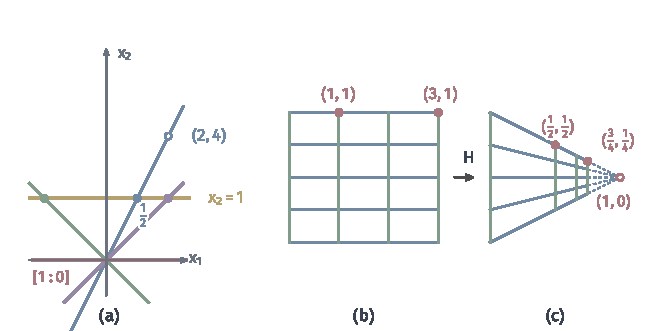
\includegraphics[width=112mm]{figures/04-spaces-measures-and-geometry/04-manifolds/matplotlib/lie-projective/figure.pdf}
  \caption{射影空间的仿射图与射影变换。(a)$\mathbb{RP}^1$的末分量图：过原点的直线与黄线$x_2=1$的交点给出坐标，蓝线是$[2:4]$，坐标为$\frac12$；红色水平线$[1:0]$不与黄线相交，是这张图的无穷远点。(b)平面上的方格，蓝线$v=$常数，绿线$u=$常数，红点是$(1,1)$与$(3,1)$。(c)方格在$\bm H$下的像（横向比例放大）：绿线仍是竖线，蓝线不再平行，延长后交于$(1,0)$。}
  \label{fig:lie-projective}
\end{BookInlineFigure}

在射影平面$\mathbb{RP}^2$中，非零系数向量$\bm\ell\in\mathbb R^3$确定直线$\{[\bm x]:\bm\ell^\top\bm x=0\}$，$\bm\ell$与它的非零倍数确定同一条直线。在$x_3=1$的图中它就是$\ell_1u+\ell_2v+\ell_3=0$。

两条平行线$u=0$与$u=1$的系数分别是$(1,0,0)^\top$与$(1,0,-1)^\top$。同时满足两个方程，第一个方程给出$x_1=0$，第二个方程再给出$x_3=0$，所以交点的齐次坐标是$[0:1:0]$，在这张图之外。平行线在射影平面中交于一个无穷远点。

\paragraph{射影变换}
可逆线性映射把过原点的直线映成过原点的直线，所以诱导出射影空间上的变换。

\begin{definition}[射影变换]
\label{def:lie-projective-transformation}
对$\bm H\in\mathrm{GL}(n+1,\mathbb R)$，映射$[\bm x]\mapsto[\bm H\bm x]$称为$\mathbb{RP}^n$上的\term{射影变换}（projective transformation）。
\end{definition}

它不依赖代表元，因为$\bm H(\lambda\bm x)=\lambda\bm H\bm x$；$\bm H\bm x\neq\bm0$由$\bm H$可逆保证。在仿射图中它是有理函数，因而光滑，逆变换由$\bm H^{-1}$给出，所以是微分同胚。$\bm H$与$c\bm H$（$c\neq0$）给出同一个变换，所以射影变换组成的群是$\mathrm{GL}(n+1,\mathbb R)$按非零数量矩阵取商，参数个数为$(n+1)^2-1$，平面的情形$n=2$有$8$个自由度。

射影变换保持点在线上的关系。若点按$\bm x'=\bm H\bm x$变换，令直线系数按$\bm\ell'=\bm H^{-\top}\bm\ell$变换，则
\[
\bm\ell'^\top\bm x'=\bm\ell^\top\bm H^{-1}\bm H\bm x=\bm\ell^\top\bm x,
\]
所以$\bm x$在$\bm\ell$上当且仅当$\bm x'$在$\bm\ell'$上。

它一般不保持长度、角度和平行。例如
\[
\bm H=\begin{bmatrix}1&0&0\\0&1&0\\1&0&1\end{bmatrix},\qquad
(u,v)\longmapsto\Bigl(\frac{u}{u+1},\frac{v}{u+1}\Bigr)\quad(u\neq-1).
\]
点$(1,1)$变成$(\frac12,\frac12)$，点$(3,1)$变成$(\frac34,\frac14)$。

这两个像点的连线延长后经过$(1,0)$，因为直线$v=1$上的点都是$\frac{v}{u+1}=\frac1{u+1}=1-\frac{u}{u+1}$，满足$v'=1-u'$。所有水平线$v=c$的像都经过$(1,0)$，图~\ref{fig:lie-projective}(b)(c)中平行的蓝线在像中汇聚到这一点。这个点是平行线在无穷远处交点的像：$\bm H(1,0,0)^\top=(1,0,1)^\top$。

直线$u=-1$上的点仍有合法的齐次像，只是像的第三分量为零，落到末分量图的无穷远处。所以“除以末分量”只能在它非零时进行，不能当作全局的线性运算。

刚体变换是射影变换的特例：式~\eqref{eq:lie-homogeneous-pose}中的$\bm T$底行为$(0,0,0,1)$，把末分量为$1$的点仍送到末分量为$1$的点，保持无穷远点组成的集合。由给定的点对应估计一个未知的$\bm H$，需要消去未知的比例并处理退化配置，这是第~\ref{chap:spatial-map-estimation}章的问题。

\subsection{Grassmann空间}
\label{sec:lie-grassmann}

射影空间研究$\mathbb R^{n+1}$中的一维子空间。数据分析中常常关心更高维的子空间，例如一组样本主要分布在哪个$k$维子空间附近。子空间本身是一个几何对象，但要计算它，通常得选一组基，把它记为矩阵；不同的基给出同一个子空间。

\paragraph{用基表示子空间}
设$\bm Y\in\mathbb R^{n\times k}$的列线性无关，它的列空间是一个$k$维子空间。若$\bm A\in\mathrm{GL}(k,\mathbb R)$，则$\bm Y\bm A$的各列是$\bm Y$各列的线性组合，并且仍线性无关，所以列空间不变。反过来，若$\bm Y,\bm Y'$列空间相同，则$\bm Y'$的每一列都能唯一地写成$\bm Y$各列的组合，即$\bm Y'=\bm Y\bm A$，且$\bm A$可逆。所以“同一子空间”恰好是$\mathrm{GL}(k,\mathbb R)$按右乘作用的轨道，这个对象因此可以用商来定义。

\begin{definition}[Grassmann空间]
\label{def:lie-grassmann}
$\mathbb R^n$中全体$k$维线性子空间组成的集合记为$\mathrm{Gr}(k,n)$，称为\term{Grassmann空间}（Grassmannian）。
\end{definition}

列满秩的$n\times k$矩阵组成$\mathbb R^{n\times k}$中的开集，记为$F$，$\mathrm{GL}(k,\mathbb R)$按$\bm A\cdot\bm Y=\bm Y\bm A^{-1}$在其上作用。作用是自由的：$\bm Y\bm A=\bm Y$与列满秩推出$\bm A=\bm I$。

作用也是适当的。设$K\subset F\times F$紧，若$(\bm Y\bm A^{-1},\bm Y)\in K$，记$\bm Y'=\bm Y\bm A^{-1}$，由列满秩解出
\[
\bm A=(\bm Y'^\top\bm Y')^{-1}\bm Y'^\top\bm Y,\qquad
\bm A^{-1}=(\bm Y^\top\bm Y)^{-1}\bm Y^\top\bm Y'.
\]
两个公式的右边在紧集$K$上连续，所以$\bm A$与$\bm A^{-1}$都有界，原像落在$\mathrm{GL}(k,\mathbb R)$的紧子集与$K$的投影之积内，又是闭集，从而是紧集。

由定理~\ref{thm:lie-quotient-manifold}，$\mathrm{Gr}(k,n)$是光滑流形，维数为$nk-k^2=k(n-k)$。$k=1$时它就是$\mathbb{RP}^{n-1}$，维数$n-1$。

\paragraph{用标准正交基表示}
计算中更常用标准正交基。满足$\bm Y^\top\bm Y=\bm I_k$的$n\times k$矩阵全体称为\term{Stiefel流形}（Stiefel manifold），记为$\mathrm{St}(k,n)$。与定理~\ref{thm:lie-orthogonal-group-manifold}的证明相同，约束$\bm Y^\top\bm Y=\bm I_k$取值于$\mathrm{Sym}(k)$且以$\bm I_k$为正则值，所以$\mathrm{St}(k,n)$的维数是$nk-k(k+1)/2$。

同一子空间的两组标准正交基只差一个正交矩阵，$\bm Y'=\bm Y\bm Q$，$\bm Q\in\mathrm O(k)$。紧群$\mathrm O(k)$的这一作用自由且适当，于是
\begin{equation}
 \mathrm{Gr}(k,n)\cong\mathrm{St}(k,n)/\mathrm O(k).
 \label{eq:lie-grassmann-stiefel}
\end{equation}
维数核对：
\[
nk-\frac{k(k+1)}2-\frac{k(k-1)}2=k(n-k),
\]
与上一段的结果一致。$k=n$时$\mathrm{St}(n,n)=\mathrm O(n)$，$\mathrm{Gr}(n,n)$只有一个点。

\paragraph{子空间与标架的区别}
标准正交基$\bm Y$称为一个标架，它比子空间多记录了$k(k-1)/2$个自由度，即在子空间内部怎样选取各轴。图~\ref{fig:lie-grassmann-frames}(a)中$\mathbb R^3$的一张平面对应两组不同的标架，它们是$\mathrm{St}(2,3)$中两个不同的点，却是$\mathrm{Gr}(2,3)$中同一个点。

消除这些自由度的一种方式是改用正交投影矩阵$\bm P=\bm Y\bm Y^\top$。对$\bm Q\in\mathrm O(k)$，
\[
(\bm Y\bm Q)(\bm Y\bm Q)^\top=\bm Y\bm Q\bm Q^\top\bm Y^\top=\bm Y\bm Y^\top,
\]
所以$\bm P$只依赖子空间；反过来，$\bm P$的列空间就是该子空间。于是$\mathrm{Gr}(k,n)$可以与秩为$k$的对称幂等矩阵一一对应，这个矩阵集合是
\[
\{\bm P:\bm P^\top=\bm P,\ \bm P^2=\bm P,\ \operatorname{tr}\bm P=k\}.
\]

切方向也要区分。在标架$\bm Y$处，Stiefel流形的切向量$\bm\Delta$满足$\bm Y^\top\bm\Delta+\bm\Delta^\top\bm Y=\bm0$。设$\bm Y_\perp$的列是正交补的一组标准正交基，切向量分解为
\[
\bm\Delta=\bm Y\bm\Omega+\bm Y_\perp\bm B,\qquad \bm\Omega^\top=-\bm\Omega .
\]

形如$\bm Y\bm\Omega$的方向只在子空间内部转动标架，不改变子空间，称为竖直方向；形如$\bm Y_\perp\bm B$（满足$\bm Y^\top\bm\Delta=\bm0$）的方向才真正把子空间推向别处，称为水平方向。水平方向组成的线性空间维数为$(n-k)k$，恰好是$\mathrm{Gr}(k,n)$的维数，可以作为子空间处切空间的具体表示。

取$n=3$，$k=2$，$\bm Y=[\bm e_1,\bm e_2]$。竖直方向和水平方向各取一个例子：
\[
\bm\Delta_v=[\bm e_2,\ -\bm e_1],\qquad
\bm\Delta_h=[\tfrac12\bm e_3,\ \bm0].
\]
前者对应$\bm\Omega=\begin{bmatrix}0&-1\\1&0\end{bmatrix}$，后者对应$\bm B=(\tfrac12,0)$，它把平面绕$\bm e_2$轴倾斜。图~\ref{fig:lie-grassmann-frames}(b)画出了这两种方向。

\begin{BookInlineFigure}
  \centering
  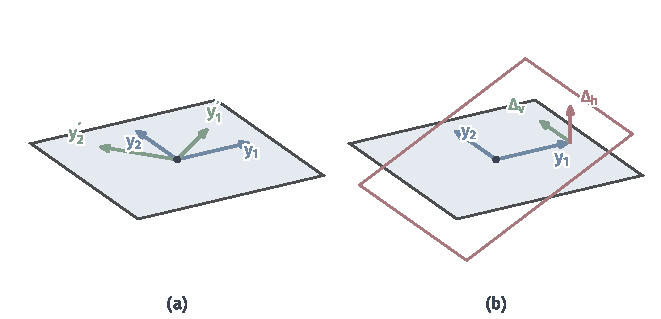
\includegraphics[width=112mm]{figures/04-spaces-measures-and-geometry/04-manifolds/matplotlib/lie-grassmann-frames/figure.pdf}
  \caption{$\mathbb R^3$中的平面与标架。(a)同一张平面的两组标准正交基，蓝色$\bm Y$与绿色$\bm Y\bm Q$相差平面内转动$38^\circ$，它们是$\mathrm{St}(2,3)$的两个点、$\mathrm{Gr}(2,3)$的同一个点。(b)标架$\bm Y=[\bm e_1,\bm e_2]$处的两种切向量。绿箭头是竖直方向$\bm\Delta_v$的第一列（画成$0.75$倍长），只转动标架；红箭头是水平方向$\bm\Delta_h$的第一列，把平面倾斜到红框所示的新平面。}
  \label{fig:lie-grassmann-frames}
\end{BookInlineFigure}

\paragraph{局部坐标}
子空间也有类似仿射图的坐标。若一个$k$维子空间与后$n-k$个坐标组成的子空间只交于零，它就有唯一的一组基写成$\begin{bmatrix}\bm I_k\\\bm B\end{bmatrix}$，$\bm B\in\mathbb R^{(n-k)\times k}$。$\bm B$的$k(n-k)$个元素就是这类子空间的坐标。$k=1$时它正是射影空间的首分量仿射图。不满足这个条件的子空间，换一组$k$个坐标的位置即可同样处理。

以正交约束或子空间为未知量的优化，要把这里的切方向、商结构与回到流形的更新方式结合起来，这是\BookChapterRef{chap:manifold-optimization}{卷五第25章“流形优化”}的内容；本节只说明这些未知量是什么对象、有多少自由度。

\section{本章小结}
\label{sec:lie-summary}

本章开头问：怎样说清一个计算“不受旋转影响”还是“随旋转同步变化”，以及怎样在只有三个自由度的旋转上做计算而不破坏约束。第一个问题的回答分两层。群只规定变换怎样复合：结合律、单位元和逆元保证变换可以接连施加和撤销，复合的次序一般不能交换。子群是对运算封闭的允许变换，而不是任意子集；同态保持复合，它的核记录丢失了哪些区分，像记录实际表示了哪些元素，元素个数相同的两个群未必同构。

群作用再规定每个变换怎样改变一个具体对象。同一个群可以作用在点、点云和图像上，公式各不相同，都要核对单位元与复合两条规则。轨道收集通过变换可以互相到达的对象，稳定子收集不改变给定对象的变换，二者分别是对象集合与群的子集，由陪集一一联系。在输入与输出的作用都给定后，不变映射在每条轨道上取常值，等变映射的输出按指定规则随输入变化；重心对置换不变、对旋转等变，距离矩阵对旋转不变、对置换在共轭作用下等变。不变是输出作用平凡时的等变，不变性也不保证保留了区分轨道所需的信息。

第二个问题由矩阵Lie群回答。$\mathrm{GL}(n,\mathbb R)$是开集，$\mathrm O(n)$与$\mathrm{SO}(n)$是正则水平集，乘法与求逆都光滑，左平移把单位元处的切空间搬到每一点。单位元处的切空间即Lie代数，可以做线性组合，交换子记录变换的不交换；它的元素是速度，不是群中的变换。矩阵指数由幂级数定义，把Lie代数方向变成单参数子群，并在单位元附近给出局部坐标，但一般既不单射也不满射。它只依赖群结构，与依赖度量的黎曼指数是两回事，只在$\mathrm{SO}(n)$配Frobenius度量这类特殊情形中吻合。

三维旋转没有全局无奇异的三参数坐标，这由$\mathrm{SO}(3)$的紧性直接推出。旋转矩阵直接作用于向量；轴角由Rodrigues公式给出，在半圈旋转与恒等旋转处有冗余，旋转向量在模长小于$\pi$的开球内是局部坐标；Euler角在万向节锁处秩下降，那是坐标的奇异而非旋转的退化。单位四元数以乘法完成复合，在每一点附近都给出正常坐标，代价是$q$与$-q$表示同一旋转，这一双覆盖不是额外的物理自由度。刚体位姿把旋转与平移合成$\mathrm{SE}(3)$，复合时前一次的平移要随后一次的旋转转动，方向不受平移影响；同一个齐次矩阵既可读作主动变换，也可读作坐标系换算。

最后，多种记录代表同一对象时，用群作用把同一轨道合并。商集合与商拓扑总能定义，但光滑结构需要条件：自由且适当的光滑作用给出维数为$\dim M-\dim G$的商流形，闭子群给出齐性空间，例如$\mathrm{SO}(3)/\mathrm{SO}(2)\cong S^2$；$\mathrm{SO}(2)$作用于平面的商有端点，无理旋转的商不是Hausdorff空间，都说明这些条件不能省略。射影空间合并非零倍数，用仿射图记录点、用可逆矩阵诱导射影变换；Grassmann空间合并张成同一子空间的不同基，标架比子空间多出的自由度可以用投影矩阵或水平方向消去。由点对应实际估计刚体变换与射影变换，在第~\ref{chap:spatial-map-estimation}章研究；正交矩阵与子空间上的优化算法留给卷五。

